\documentclass[../thesis.tex]{subfiles}

\begin{document}

%% There are two major categories of localization. Visual-based approaches for pose estimation has experienced great improvements, but it is still difficult to achieve industry-standard precision. Particularly, learning-based approaches require large datasets, which makes them less applicable in manufacturing for parts with irregular shapes. For touch-based approaches using tactile sensors, the object is often assumed to be a rigid body. In order to handle objects with complex shape, prior information of the object shape is always required, and most previous work assumes that the geometry (CAD) model will match the real object exactly.

Many robotic tasks require precisely localizing an object, for which tactile sensing is an appealing sensing modality.
As motivation, consider touch localization of a partially manufactured part that requires additional machining operations.
In order to handle objects with complex shape, prior information of the object shape is used, and most previous work assumes that the geometry (CAD) model will match the real object exactly.


However, during the manufacturing and assembly processes there are tolerances between different sections of the assembly. A \textit{datum} is defined as a geometric constraint within the object that is used as the reference to define the location of one section of the part with respect to another section. The tolerance is the allowed deviation of the actual manufactured dimensions from the nominal designed dimensions.
It is assumed a part can be divided into precisely manufactured sections, and the introduced method focuses on handling errors due to imprecise machining over large distances and non-critical components, as well as assembly tolerances.
%% One example of the tolerance is the distance between two parallel datum planes: the distance could be $1.0 \pm 0.1mm$. 

The introduction of tolerance increases the degrees of freedom (DOFs) of the system, as prior to measurement the true dimensions of the full part are unknown. 
These internal DOFs can be modeled as transformations with uncertainty between sections of the object.
For objects with internal tolerances, perfectly localizing a single datum will not necessarily reduce the uncertainty of the full system sufficiently to perform the desired task.
On the other hand, it is usually only necessary to localize a subset of the sections of an object.

\begin{figure}
  \centering
  \begin{subfigure}[b]{0.4\linewidth}
    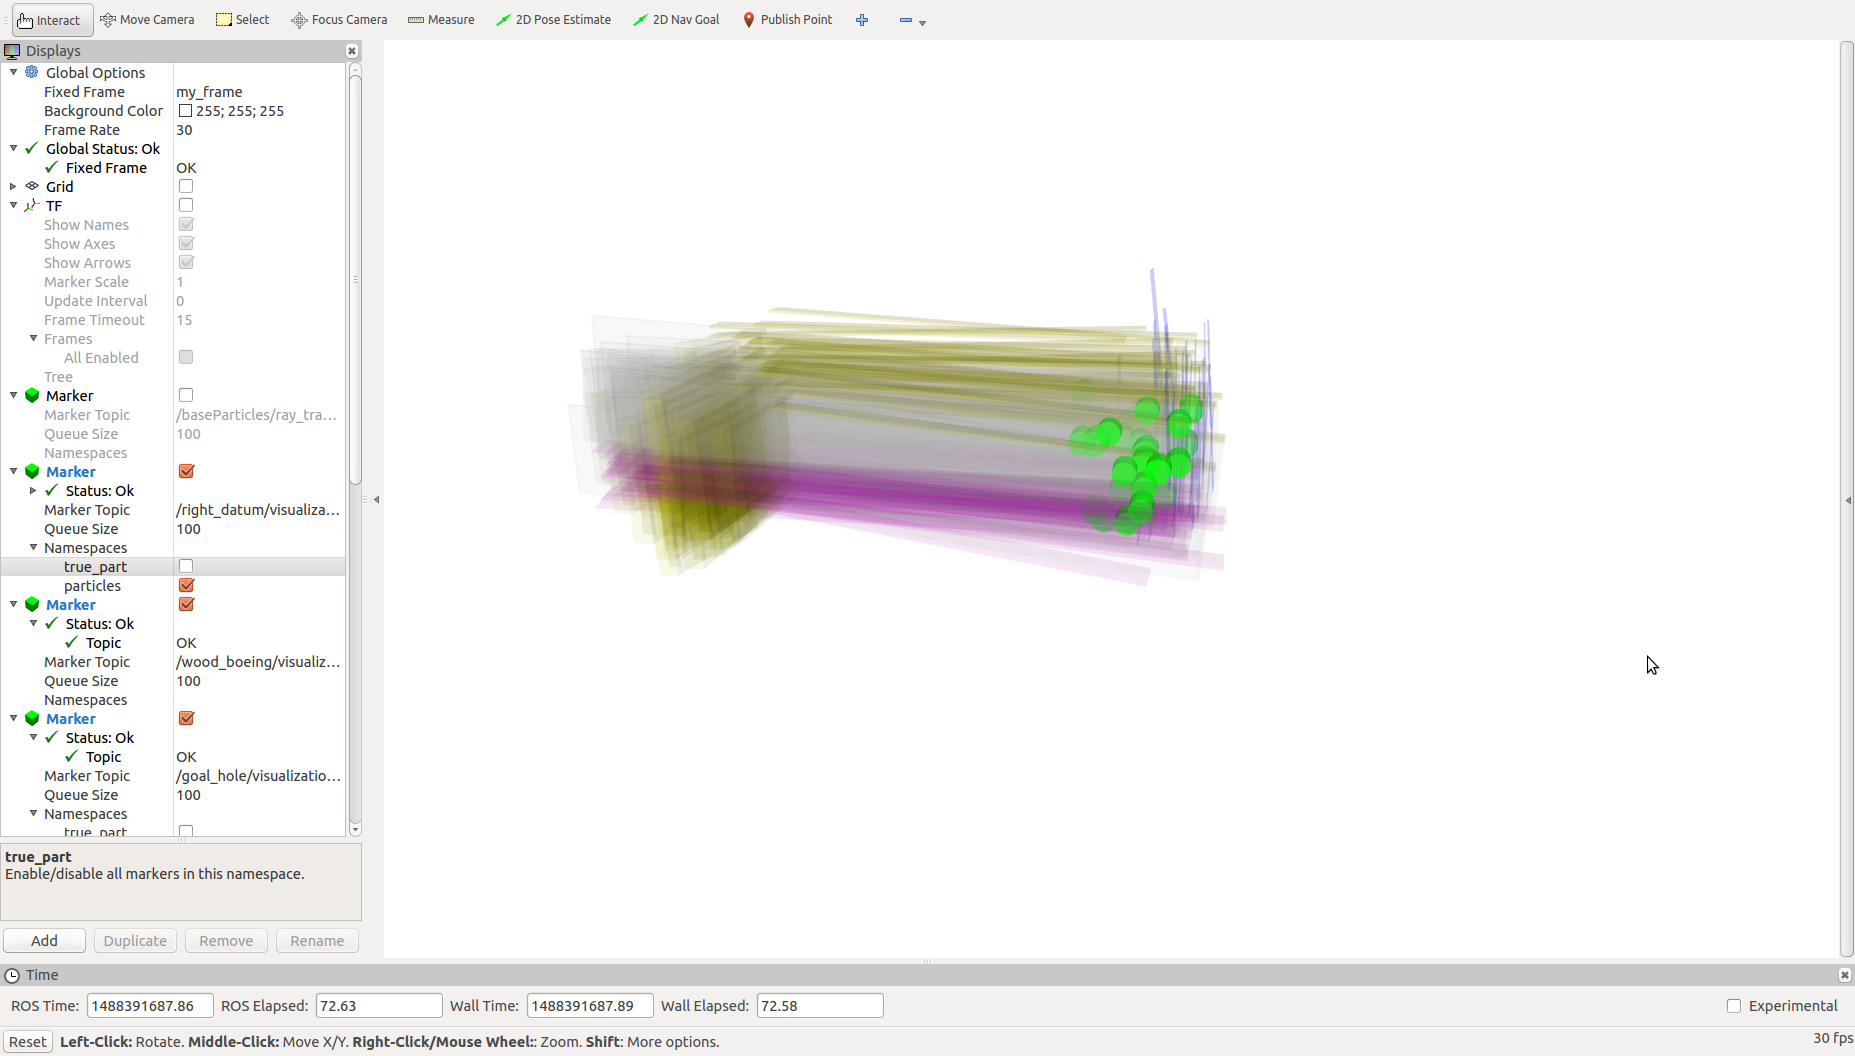
\includegraphics[width=\linewidth, clip, trim=8in 6in 8.5in 4in]{./Localization/UnlocalizedBelief}
    \caption{Initial belief}
    \label{fig:FullBelief:Unlocalized}
  \end{subfigure}
  \hfill
  \begin{subfigure}[b]{0.4\linewidth}
    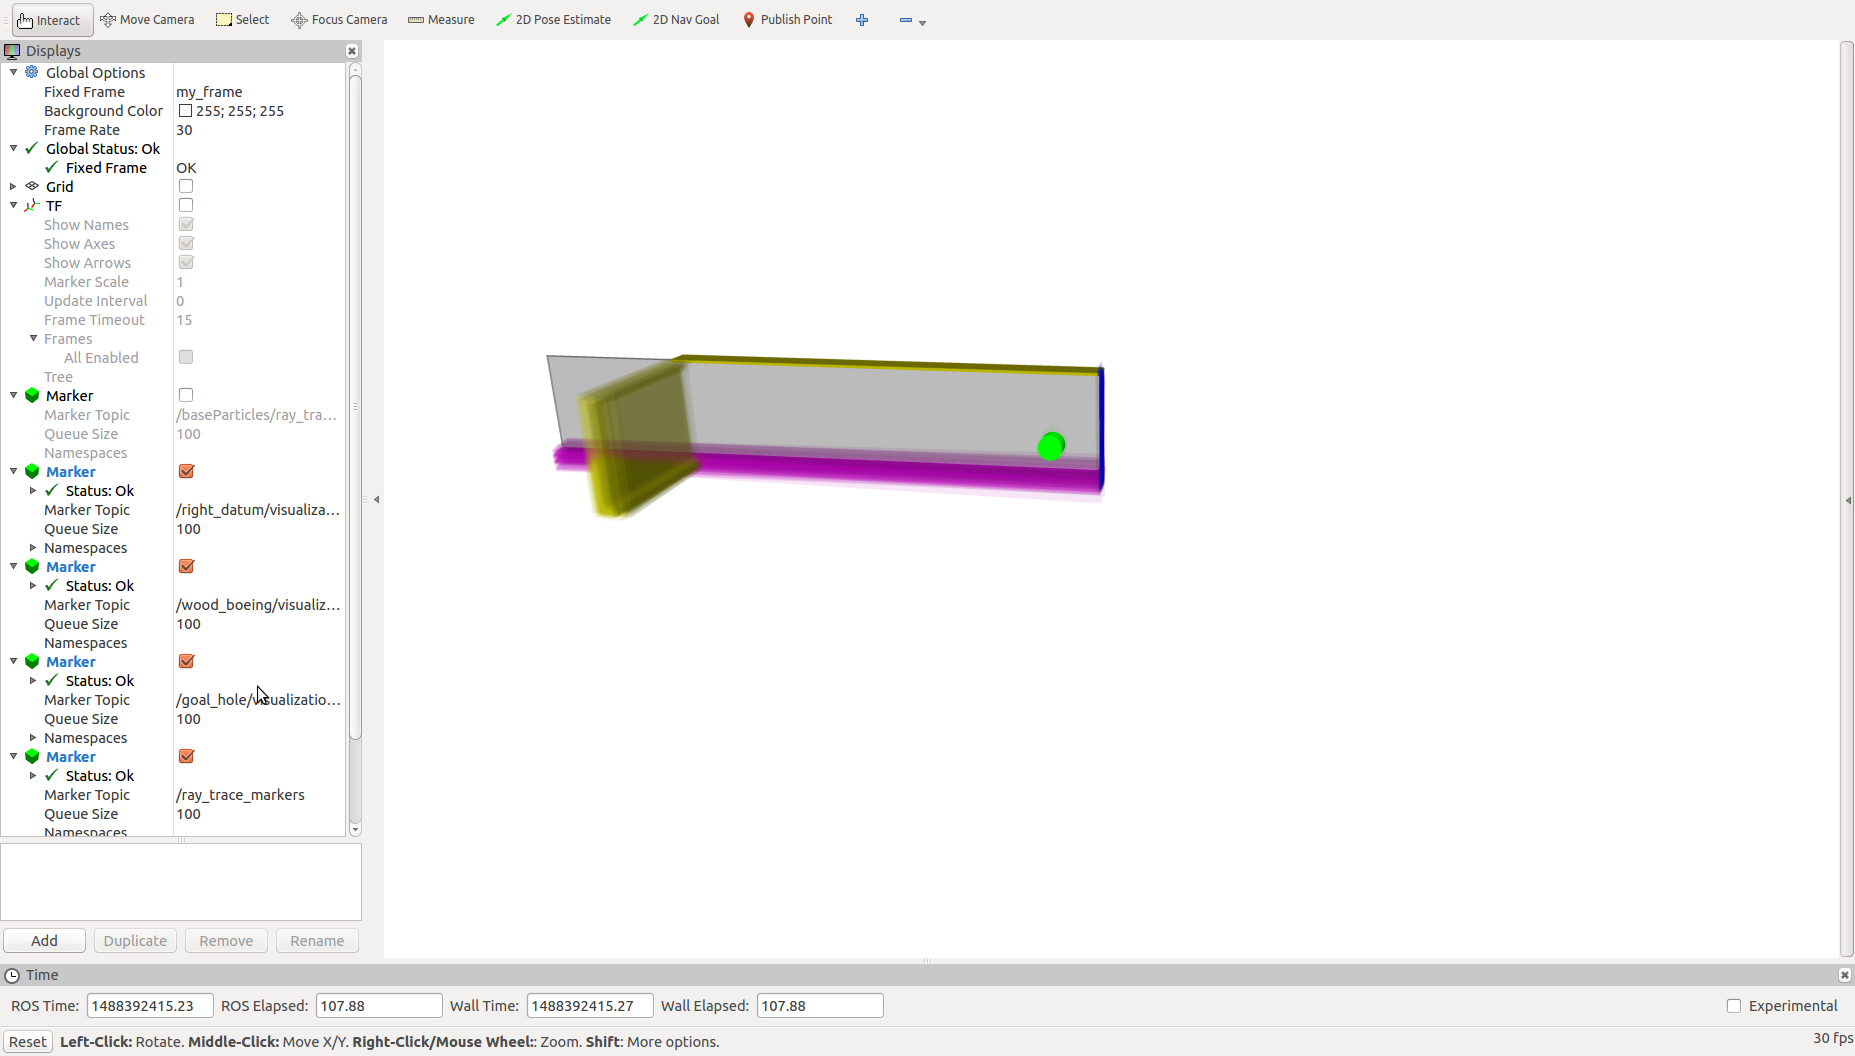
\includegraphics[width=\linewidth, clip, trim=7in 7in 10in 4in]{./Localization/LocalizedBelief}
    \caption{Belief after localization of goal feature (green cylinder)}
    \label{fig:FullBelief:Localized}
  \end{subfigure}
  \caption{
    Visualization of the belief of the pose of all sections of the part\\
\protect\subcap{fig:FullBelief:Unlocalized}: The prior belief of the poses before localization. The uncertainty of the goal feature is too high to perform the task.\\ 
\protect\subcap{fig:FullBelief:Localized}: The belief of the poses after performing measurements to localize the goal feature. The pose of the goal feature is now known well enough to perform the task. Although the bottom edge (purple) and perpendicular section still have noticeable error, precise localization of these features is not needed.
}
  \label{fig:FullBelief}
\end{figure}

In this localization problem, the task is to estimate the pose of a goal feature given multiple measurements obtained through probing. 
These probing measurements are modeled as a Markov process, where each measurement corresponds to a single action/observation pair. 
This model eliminates the need to store all of the past measurements. 
A particle filter numerically stores and updates the belief \cite{Thrun2000a}.

Figure \ref{fig:FullBelief} shows a visualization of the initial (\ref{fig:FullBelief:Unlocalized}) and final (\ref{fig:FullBelief:Localized}) beliefs of the poses of the sections of the object.
The task is to drill a hole, shown as a green cylinder, at a specific location defined by offsets from other sections.
Internal tolerances prevent simply treating the entire system as a rigid body.


This chapter first considers rigid-body particle filtering for high-precision localization (section \ref{sec:rigid_body}), which overcomes the particle starvation problem and serves as the basis for this chapter \cite{Saund2017}. 
The datum-based particle filter is then introduced to generalize this rigid-body approach for objects with coupled rigid sections (section \ref{sec:datum}).
Two related but different approaches are proposed for this problem.
The first approach maintains a single particle filter system that stores the full joint distribution of the coupled datums, while the second approach simplifies the relationships by assuming independence between the distribution of the internal transformations and the pose of the sections, and models the system using separate coupled particle filters. 

This chapter then generalizes the technique of choosing informative measurement actions to accommodate objects with coupled sections.
To achieve this, many potential measurement actions are sampled and the action with the highest expected information gain is selected. 
Fully predicting the information gain over the continuous belief is computationally expensive, so similar to other approaches \cite{Javdani2013} this work involves a fast approximation for information gain that takes advantage of the discretized belief from the particle filter (section \ref{sec:information gain}). 
This chapter concludes with demonstrations of the method on a simulated part (section \ref{sec:experiment}). 

\section{Current Methods for Localizing Objects Using Contact Sensors}

%Particle filter has been widely used in localization tasks since its introduction.
%
%%PLACE HOLDER
%Particle filters, touch measurements, and maximal information gain measurement selection have all been used in localization tasks. 
%In particular the recent DARPA ARM-S competition led to progress with robotic arms localizing and grasping objects. 

% Touch is considered one of the most accurate ways of perception. 
%% Humans are capable of localizing objects with complex shape using sense of touch. 
%% However, for robots, localization using contact sensors is a classic problem, as it requires robots to reason in high-dimensional configuration space. 

Recently, there have been a variety of approaches that allow robots to localize objects solely with contact sensors. Different contact sensors have been explored and developed, including basic binary sensors, 6-axis force and torque sensors \cite{del2012control}, soft tactile sensor arrays \cite{hammond2012soft}, and bio-inspired fingertips \cite{fishel2012sensing}. Localization with laser sensors has also been used in the high-precision CNC localization, where a 3D point cloud is acquired in order to estimate the transformation between the actual and planned pose \cite{rajaraman2013automated}.
The localization approach presented here can be generalized to these sensors which can distinguish between contact and free-of-contact states.

Particle filters have been widely used and developed since their introduction. 
Unlike some other Bayesian estimation approaches such as Kalman filters \cite{kalman1960new}, extended Kalman filters \cite{kalman1961new} and unscented Kalman filters \cite{julier1997new}, particle filters can easily model non-Gaussian and multi-modal probability distribution. 
For touch localization, contact sensors yield a highly non-linear measurement model, and the belief can frequently become multi-modal when multiple configurations are all consistent with the measurement. 
These properties make particle filter a popular approach for touch localization tasks. 

However, particle filters will experience \textit{particle starvation} for measurements with very low uncertainty and objects with a high dimensional configuration space \cite{Thrun2000}. 
Koval introduced the Manifold Particle Filter to address this issue by implementing different sampling and weighting strategies compared to the traditional particle filters \cite{Koval2011}\cite{ Koval2013}. 
Instead of sampling particles from the process model and weighting them based on the observation, samples are directly drawn from the contact manifold, given the observation. 
This provides a fast and robust solution for objects with simple shapes. 
For complex object geometries, as in this case, direct, efficient sampling from the contact manifold becomes difficult.

Petrovskaya tackles particle starvation during touch localization by combined Monte Carlo approaches with annealing as a smoothing technique \cite{Petrovskaya2011}. 
She introduced Scaling Series algorithms for 6-DOF global tactile localization in both full-constrained and under-constrained scenarios to overcome particle starvation by adjusting particle density depending on the complexity of the posterior. 
Multiple iterations through the measurement data are used and the precision of the belief is scaled from low to high in order to avoid unnecessarily precise estimates in unlikely regions of belief space. 


All of the work mentioned so far assumes the prior information of the object geometry matches the real piece perfectly. 
Hebert et al. \cite{Hebert2013} solve a touch localization problem using a Bayes filter where an object may have additional unknown parameters describing the shape, such as a screw driver with an unknown length handle.
Measurement actions are selected using joint information gain over the object's pose and these internal parameters.
%% To the best of our knowledge, our proposed method is the first one that handles localization problems for object with coupled datums.



\section{Rigid-Body Object Localization}\label{sec:rigid_body}

The datum-based particle filter described later relies heavily on the framework and methods developed for rigid-body localization developed in \cite{Saund2017}, and this section provides an overview of the relevant details. 
The task is to determine the pose of an object by choosing and performing touch measurements, given the geometry of the object and prior belief over the distribution of poses.

The geometry of the object to be localized is stored in a STL file using a triangular mesh, defined in the \textit{part frame}. The pose of the object can then be defined as the transformation between this \textit{part frame} and the \textit{world frame} of the workspace. 
The object is assumed to be fixed in the workspace during measurement and localization, thus the configuration will not change during the localization process.

In order to estimate the true distribution of the pose, each particle in the particle filter represents a single potential pose $\particle[][i] \in SE(3)$ of the object. For a rigid body, the pose includes both translational dimensions $(x,y,z)$ and rotational Euler angles $(\alpha, \beta, \gamma)$. The state is a 6D vector $(x,y,z, \alpha, \beta, \gamma)$ in the configuration space. The particle filter updates based on a set of measurements $\measurementSet_t = \{\measurement_1, ..., \measurement_t\}$ made by the robot directly on the object. 

\subsection{Measurement Model}


A measurement action, $\maction$ is defined by a start point $\mathcal{A}_p$ for the probe and a linear trajectory vector $\mathcal{A}_v$ both in $\mathbb{R}^3$. 
The measurement value $\measurement$ is the distance the probe travels in the direction of $\mathcal{A}_v$ until contact is made. 
The point of contact can then be recovered by $A_p + \measurement \  \frac{\mathcal{A}_v}{||\mathcal{A}_v||}$. 
The entire information obtained from the measurement $t$ is $z_t = \{\maction_t, \measurement_t\}$.
Measurement error exists due to sensor error and robot uncertainty. 
%% For the robot arms and sensors used in manufacturing, the uncertainty added typically ranges from 0.1 to 1mm \cite{Saund2013}. 

\subsection{Problems with the standard particle filter} \label{sec:pfilterProblems}

A common method of updating particles based on a measurement is importance sampling \cite{Thrun2000}.
In importance sampling each particle is weighted by the probability of the measurement conditioned on the state that particle represents. 
This is usually followed by resampling, where particles are redrawn from the set of weighted particles with probability proportional to their weights. 
The effectiveness of importance sampling relies on the existence of multiple particles consistent with the measurement, such that inconsistent particles will have low weights and be unlikely to be resampled, but a sufficient number of particles will be resampled to model the true belief of the state. 

Importance sampling tends to break down in situations with accurate measurements and low densities of particles.
This is because when a measurement is consistent with the true prior belief yet no particles are consistent with the measurement, a situation called \textit{particle starvation}, resampling will yield a set of particles that does not model the true posterior belief. 
A more accurate sensor measurement is consistent with a smaller volume of state space, thus a higher density of particles is required. 
For higher dimensional state spaces and more accurate sensors the number of particles required becomes prohibitively computationally expensive. 
This leads to the counter-intuitive result that particle filters tend to perform worse as measurement accuracy increases \cite{Koval2013}. 


%% Artificially increase the measurement uncertainty alleviates particle starvation, however this loses the benefits of using an accurate sensor. 
%% Another technique uses an adaptive number of particles, as to only incur a high computational cost when it is needed. 
%% Once the particles converge updates will be fast, yet initial updates will still be slow.


\subsection{Rejection Sampling Method}
%% Our approach to update our belief based on a measurement uses rejection sampling to avoid the issues of importance sampling. 
%% We do not require a high density of particles to avoid particle starvation, and failure of rejection sampling is far easier to notice and resolve. 
%% Most importantly, we increase the limits of state dimensionality and measurement accuracy we are able to handle efficiently. 

An alternate approach is to use rejection sampling. Rejection sampling does not require a high density of particles to avoid particle starvation and failure of rejection sampling is far easier to notice and resolve. Most importantly, we can increase the limits of state dimensionality and measurement accuracy that can be handled efficiently.





Rejection sampling generates independent samples from a density $f$ by sampling from a different distribution $g$. 
A constant $M$ is determined such that $f(x) \leq M g(x) \ \forall \  x$. 
A sample $x^*$ drawn from $g(x)$ is accepted with probability $f(x^*) / {M g(x^*)}$ and rejected otherwise. 
The process is repeated until the desired number of samples has been accepted. 
We wish to sample particles from the posterior $bel(x_{t+1})$ but cannot do so directly. 
Instead we sample from our continuous prior belief $bel(x)$ and possibly reject based on the measurement.



\textit{Broad Particles}: We first reconstruct the continuous prior belief by broadening each of the particles. 
We apply a \textit{Gaussian kernel} to the particles, with the kernel covariance proportional to the covariance of the particle states. 
This reduces particle starvation, as even if no prior particle is consistent with the measurement, the continuous belief generated fills in the gaps between particles.



%% \begin{align}
%%     \Sigma = COV(\chi)\\
%%     x_{sampled} \sim \sum_i \eta \ (\chi_i + \normal{k \Sigma})
%% \end{align}

\subsection{Fast Evaluation of Sampled States}

States sampled from this continuous prior are then rejected if they are inconsistent with the measurement. 
While the formulation of rejection sampling allows us to model complicated measurement error, we implement a binary measurement model. We reject all sampled particles where the measured point is sufficiently far from all faces of the object. We define ``sufficiently far'' as more than 3 standard deviations of the sensor measurement noise.
As a low uncertainty measurement will accept only a thin manifold in state space, the probability of sampling a particle consistent with the measurement may be low, and a lot of sampling may be required, therefore we desire the rejection process to be fast.



To reduce the computational cost per sampled state we use discretized space, known as a \textit{distance field} \cite{Felzenszwalb2004}, to precompute and cache the minimum unsigned distance $D_f(p)$ from point $p$ in voxelized space to the object surface $\partial S\subseteq \mathbb{R}^3$:
\begin{align}\label{eq:7}
D_f(p) = \min_{q\in \mathbb{R}^3}(||p - q|| + f(q))\\
\label{eq:8}
f(q) = \left\{
\begin{array}{ll}
0, & \text{if }q\in\partial S\\
\infty & \text{otherwise}.
\end{array}
\right.
\end{align}

As the object is fixed during the localization process, voxelization can be done for the entire piece based on the given CAD mesh model in the precomputation step. 


\textit{Voxelization}: Voxelization is the key part to transform the mesh model to axis-aligned discretized space, which can be stored and accessed easily as a standard array. 
The array form of the CAD model can greatly facilitate the computation of the distance field, as described below. 
Each voxel is assumed to be a cube in 3D space. 
A fast 3D Triangle-Box Overlap method \cite{Akenine-Mollser2001} is used to label the voxels that overlap the mesh triangles of the object surface. 
The voxel map is then mapped to a binary-valued 3D array $f(q)$, where each value is either $0$ or $\infty$ depending on whether the corresponding voxel overlaps the object surface.

\textit{Voxelized Distance Field}: The computation of distance field $D_f(p)$ takes the input of the computed binary array $f(q)$ (Eq. \ref{eq:8}), and a linear-time algorithm for 3D distance field construction \cite{Felzenszwalb2004} is then used. The resulting distance field is also stored in an array for constant time access during the evaluation of sampled states.
 
\textit{Fast Evaluation}: Different configurations result in different poses of the object in the workspace, which makes it difficult to compute the distance field directly in the world frame. 
Instead, the computation of the voxel map and distance field is relative to the object frame, where the object is assumed fixed during the entire localization. 
Each measurement $M_t$ in the workspace is then transformed into the part frame, where the transform $T(x_{t+1})$ comes from the pose of the sampled state $x_{t+1}$. 
Therefore, by transforming back to the object frame, all measurements on this same object can share the same distance field, where the minimal unsigned distance $dist_u(M_t,S)$ between each measurement $M_t$ and the object $S(x_{t+1})$ can be obtained directly: 
\begin{align}\label{eq:9}
dist_u(M_t,S(x_{t+1})) = D_f(T(x_{t+1})^{-1}M_t)
\end{align}

%% Because $dist_u(M_t,S)$ is the distance between the center of the spherical tip of the probe and the object, when the radius $r_p$ of tip is non-zero, whether the center of the probe is inside the object becomes important. 
%% Signed distance $dist(M_t,S(x_t)$ between the probe and the object can be obtained from unsigned distance, as shown in Eq. \ref{eq:5}, by checking whether the voxel is inside or outside of the object. 
%% For the manifold shape object, ray-casting is applied from the corresponding voxel in a certain direction: if the number of intersections between the ray and mesh is odd, the voxel is inside of the object; otherwise, it's outside.

The signed distance $dist(M_t,S(x_t))$ between the probe and the object can be obtained from the unsigned distance, as shown in Eq. \ref{eq:10}, by checking whether the voxel is inside or outside of the object. 
For the manifold shape object, ray-casting is applied from the corresponding voxel in a certain direction: the voxel is inside of the object only if the number of intersections between the ray and mesh is odd
\begin{align}\label{eq:10}
dist(M_t,S(x_t) = \left\{
\begin{array}{ll}
dist_u(M_t,S(x_t) - r_p, & \text{if }M_t\notin S\\
-dist_u(M_t,S(x_t) - r_p, & \text{otherwise}.
\end{array}
\right.
\end{align}  

The unsigned distance $dist(M_t,S)$ is always $0$ in the ideal case, however, when evaluating a sampled state, only those that satisfy $|dist(M_t,S)| > T_d$ will be rejected, where $T_d$ is the tolerance selected according to the measurement uncertainty of the touch probe and the robot. If the distance is within the tolerance, ray-casting is then applied to check intersections from the start point $\mathcal{A}_p$ along the path vector $\mathcal{A}_v$ in order to determine whether the path is free of collision with other parts of the object.

When the measurement is very accurate, in order to sample enough particles from the prior belief, a large number of states will get rejected, which makes the ray-casting for all sampled states computationally expensive. Instead, early rejection is applied using a greater distance $dist_u(M_t,S) + r_p$ before the computation of signed distance. 

\subsection{Improvements on the Particle Filter}
\textit{Adaptive Voxelization}: When the workspace is large enough, it will not be feasible to compute a distance transform for the entire workspace while maintaining a sufficiently small voxel size due to the huge memory requirements. 
Instead, the distance field for each measurement is generated prior to the update. 
As the belief of the object's pose is represented as a distribution, the range of the distance field $DF$ for each measurement $M_t$ is selected so that:
\begin{align}
    \xi < \int_{T(x_t)^{-1} M_t \in DF} bel(x_{t}) dx
\end{align}

%% Where $T(x_{t-1})^{-1}M_t$ is the measurement transformed back to the object frame. 
The voxel size is adjusted accordingly while keeping the number of voxels fixed. 
When there is large uncertainty the voxels will become larger to improve the sample speed. When the uncertainty is low the precision is increased.


%% We improve the performance of our particle filter, shown in Figure \ref{fig:FasterParticles}, by adaptively choose the bandwidth and number of particles.

\textit{Adaptive Bandwidth}: The selection of the Gaussian kernel bandwidth $h$ is important during the sampling process. 
A larger bandwidth is needed when the variance of $bel(x_t)$ is large for a fixed number of particles; otherwise a smaller bandwidth is preferred to avoid over-smoothing. 
Silverman\textquotesingle s rule of thumb estimator \cite{Silverman1986} is used to dynamically adjust the bandwidth:
$h(t) = (\frac{4}{(d+2)n})^{1/(d+4)} \hat{\sigma}_t$, where $\hat{\sigma}_t$ is the standard deviation of the sampled states and number of dimensions $d = 6$.
%% $h(t) = (\frac{4}{3n})^{1/5} \hat{\sigma}_t$, where $\hat{\sigma}_t$ is the standard deviation of the sampled states.

\textit{Adaptive Sample Size}: The number of particles is determined by \textit{Kullback-Leibler divergence} (KL-divergence) which measures the difference between the sample-based maximum likelihood estimate $\hat{p}$ and the true distribution $p$:
\begin{align}
D_{KL}(\hat{p},p) = \sum_{x}\hat{p}(x)log\frac{\hat{p}(x)}{p(x)}.
\end{align}

%% Suppose that the true distribution is given by a discrete multinomial distribution with $k$ different bins with probability $p=\{p_i\}$ and the number of samples drawn from each bin $x=\{x_i\}$, the \textit{log-likelihood ratio statistic} $log\Lambda$ is��
%% \begin{align}
%% log\Lambda(\hat{p},p) = log\frac{P(x|\hat{p})}{P(x|\hat{p})}&=n\sum_{i}\hat{p}_ilog\frac{\hat{p}_i}{p_i}\\&=nD_{KL}(\hat{p},p)
%% \end{align}
%% where $log\Lambda$ converges to $\chi^2$-distribution. By substituting $log\Lambda$ with $D_{KL}(\hat{p},p)$, it can be shown that with probability $1-\delta$, the probability that KL-divergence is less than or equal to $\epsilon$ is:
%% \begin{align}
%% P(D_{KL}(\hat{p},p) \leq \epsilon) \stackrel{.}{=} P(\chi_{k-1}^2\leq 2n\epsilon) = 1-\delta
%% \end{align}
%% where $\chi_{k-1}^2$ is the $\chi^2$-distribution with $k-1$ degrees of freedom. By using Wilson-Hilferty transformation of $\chi^2$-distribution, the sample size $n$ is given by:

\begin{figure}
\centering
\begin{tikzpicture}
  \node (img) {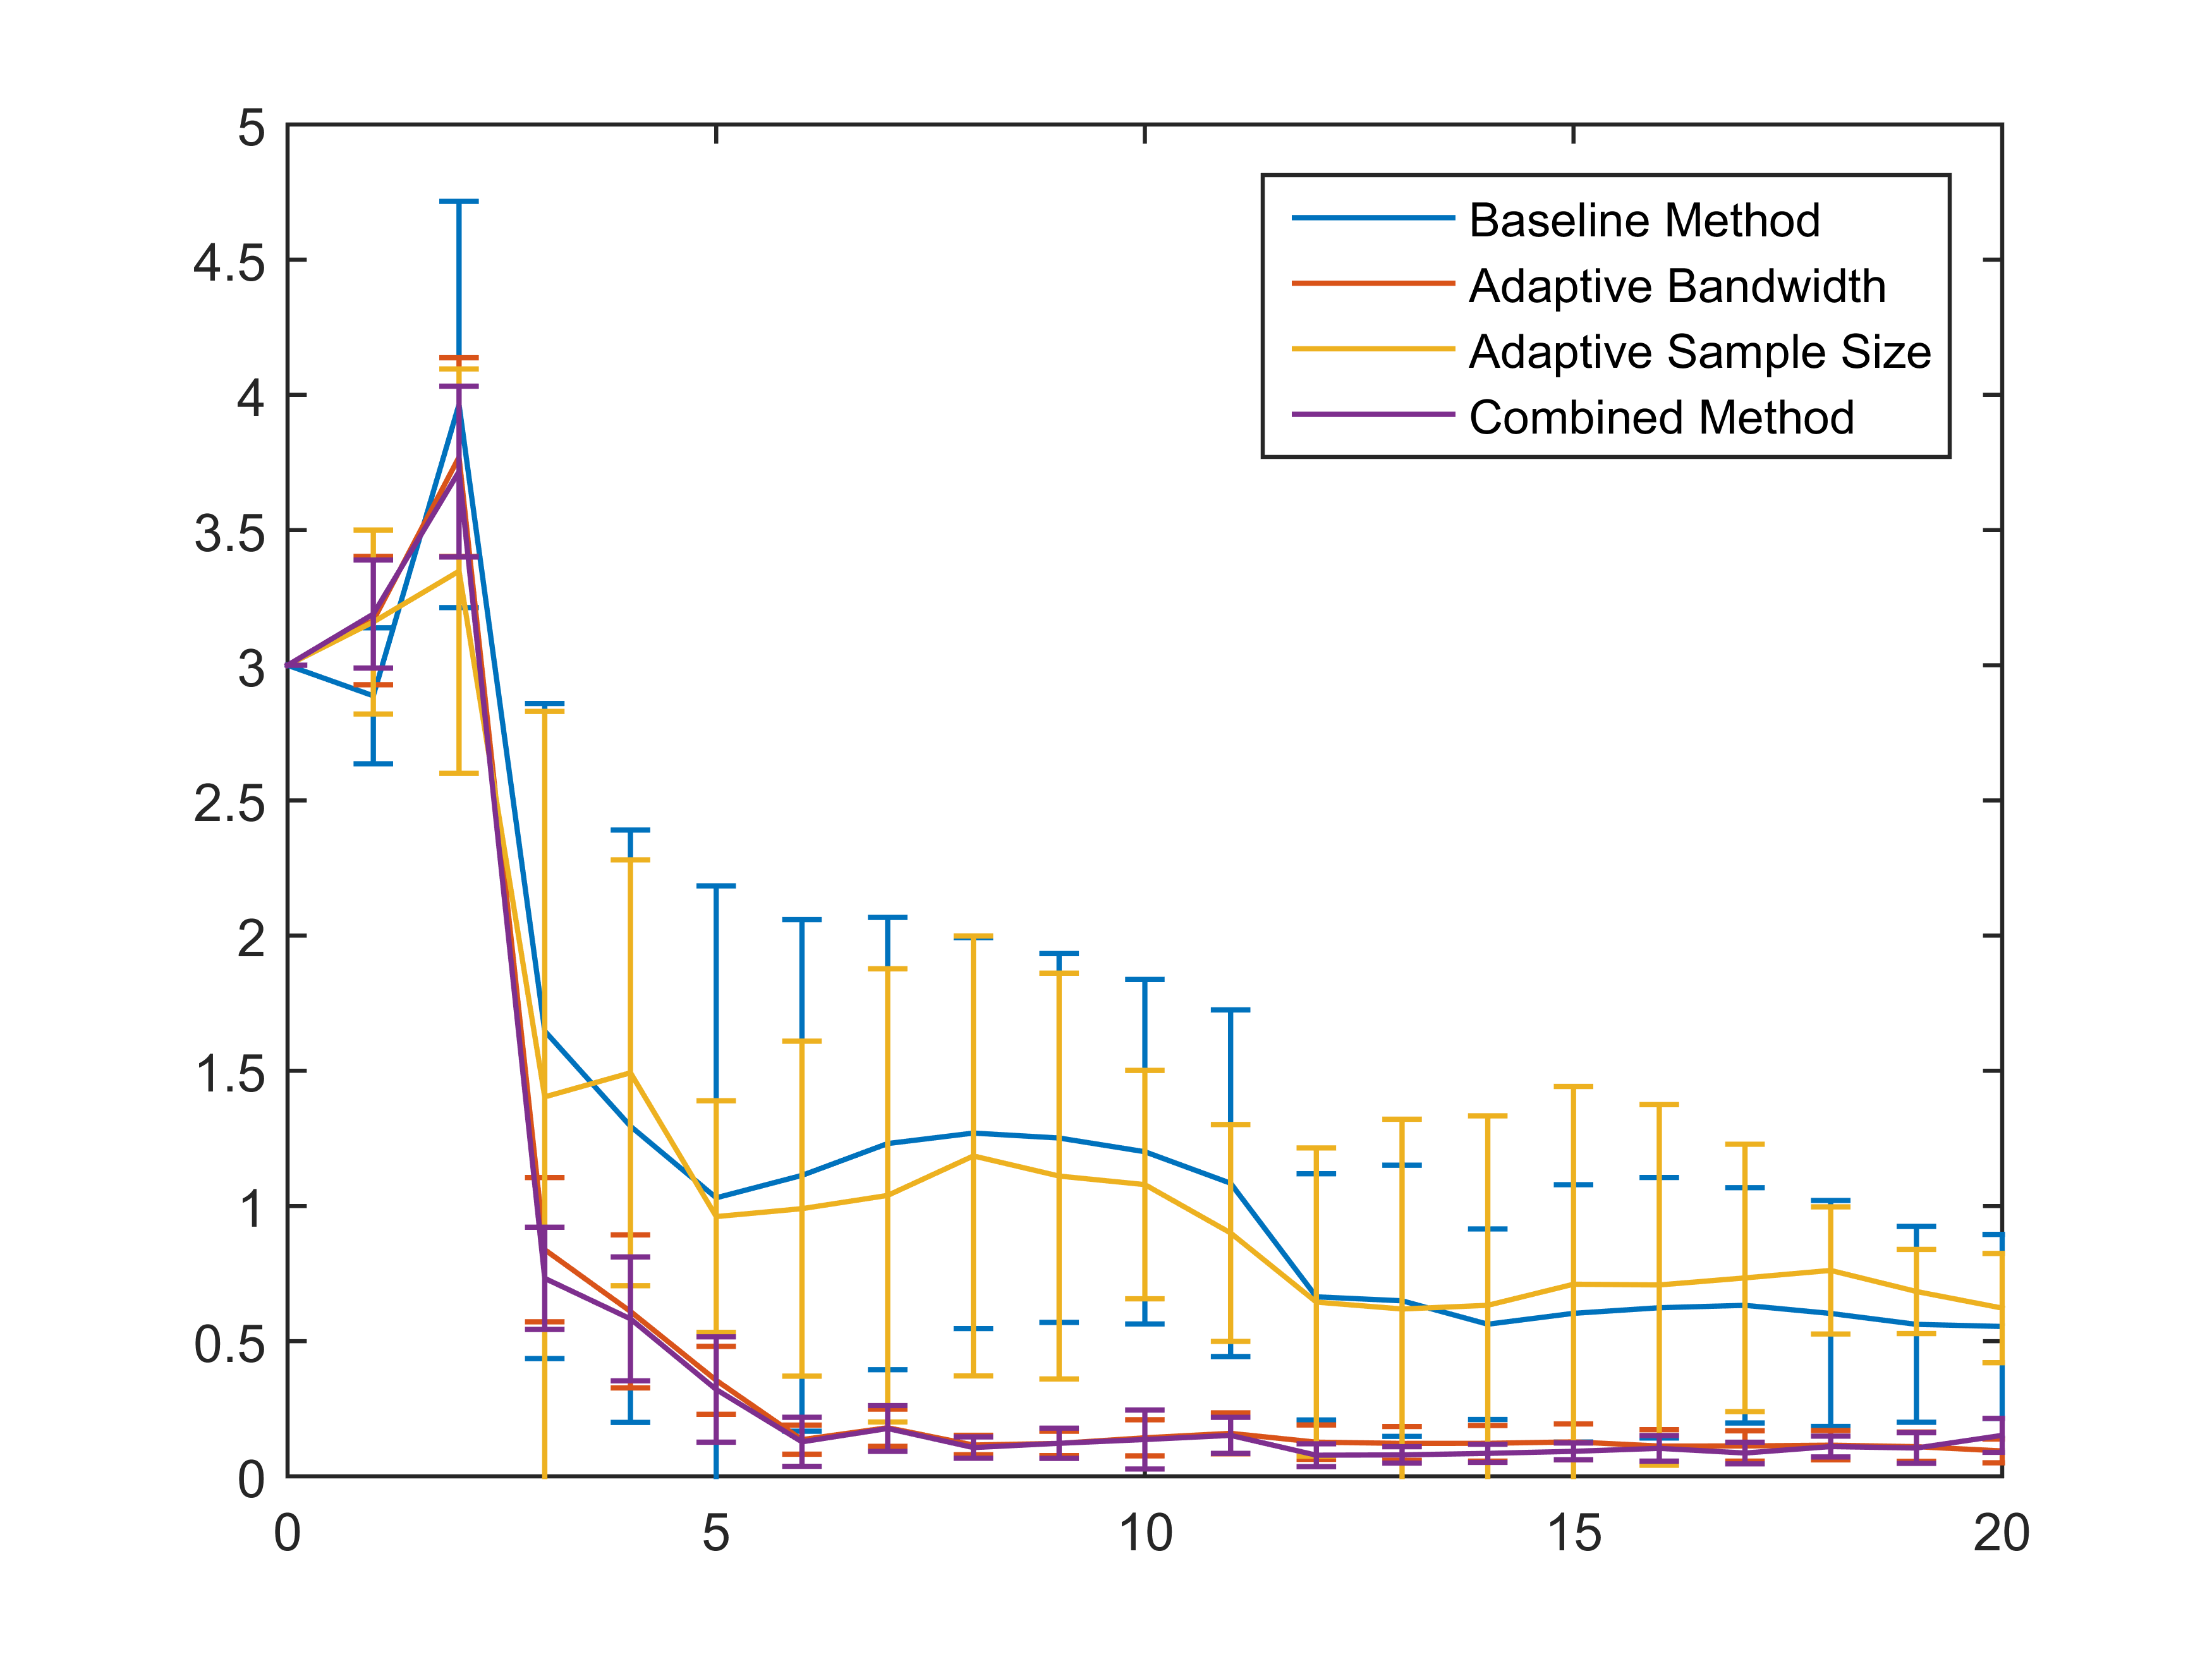
\includegraphics[width=.5\linewidth]{./Localization/diff_trans_method}};
  \node[left=of img, node distance=0cm, rotate=90, anchor=center,yshift=-1cm] 
       {Translational Error (cm)};
\end{tikzpicture}
\begin{tikzpicture}
  \node (img) {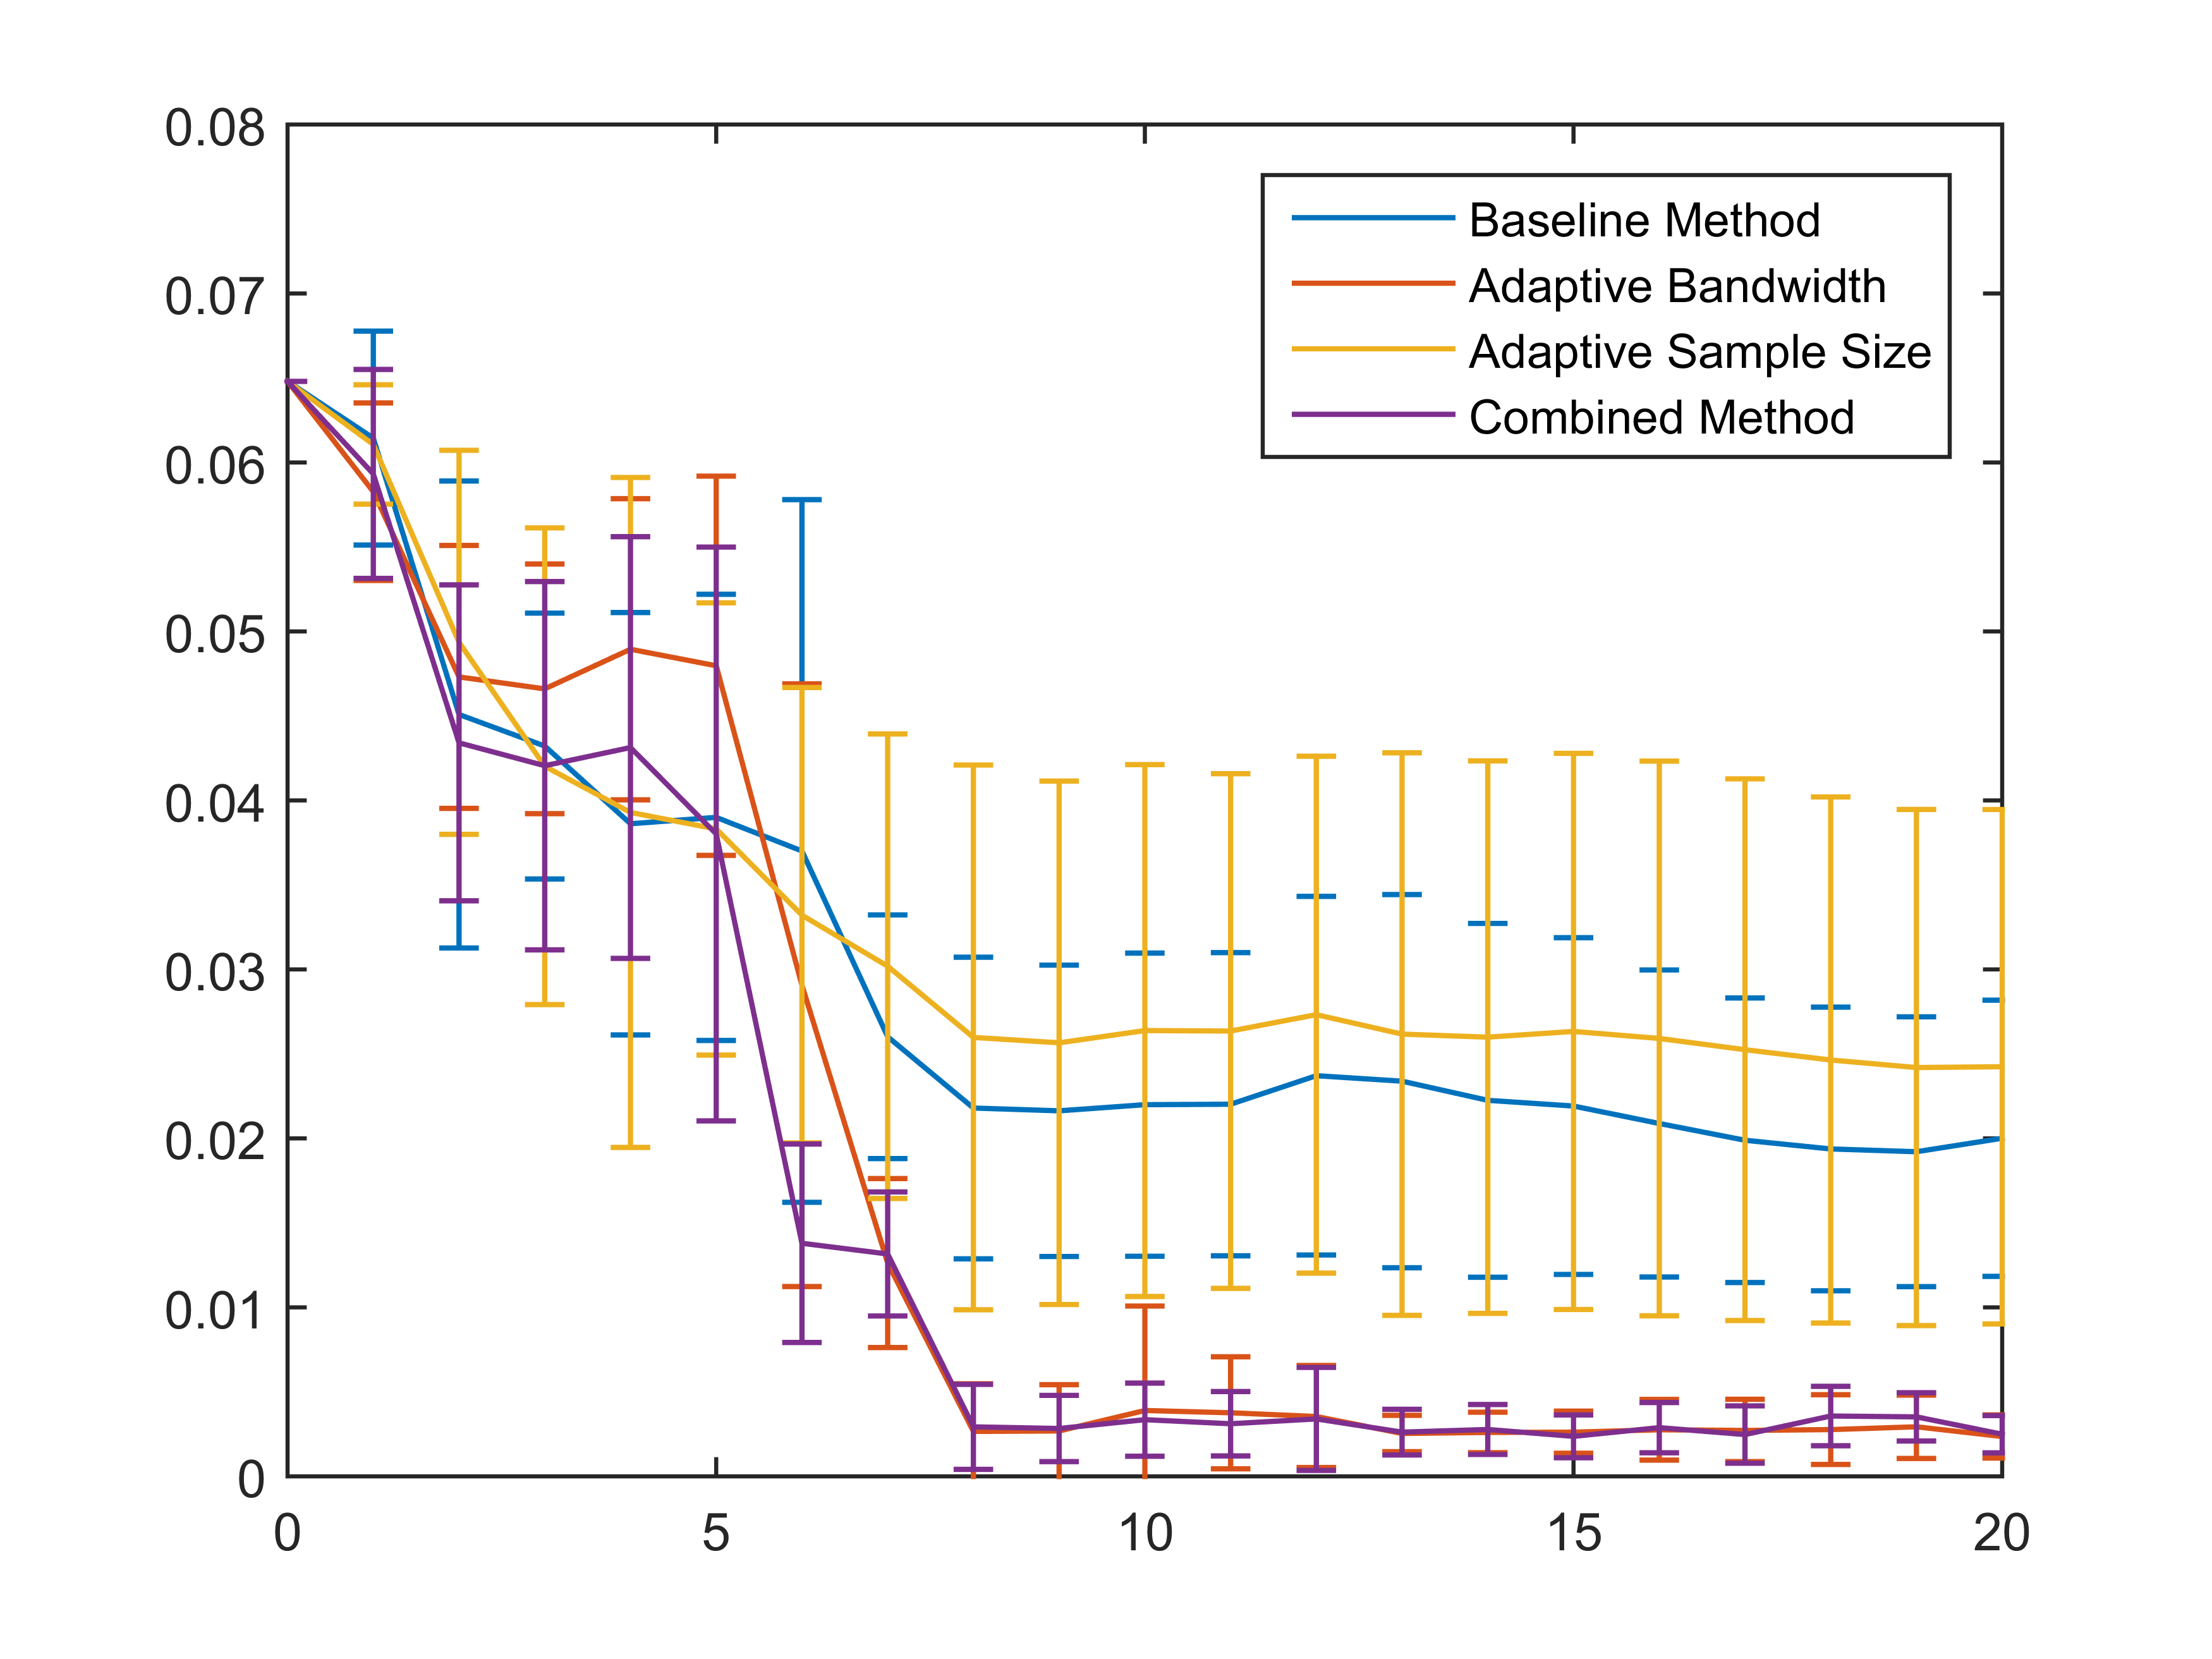
\includegraphics[width=.5\linewidth]{./Localization/diff_rot_method}};
  \node[left=of img, node distance=0cm, rotate=90, anchor=center,yshift=-1cm] 
       {Rotational Error (rad)};
\end{tikzpicture}
\begin{tikzpicture}
  \node (img) {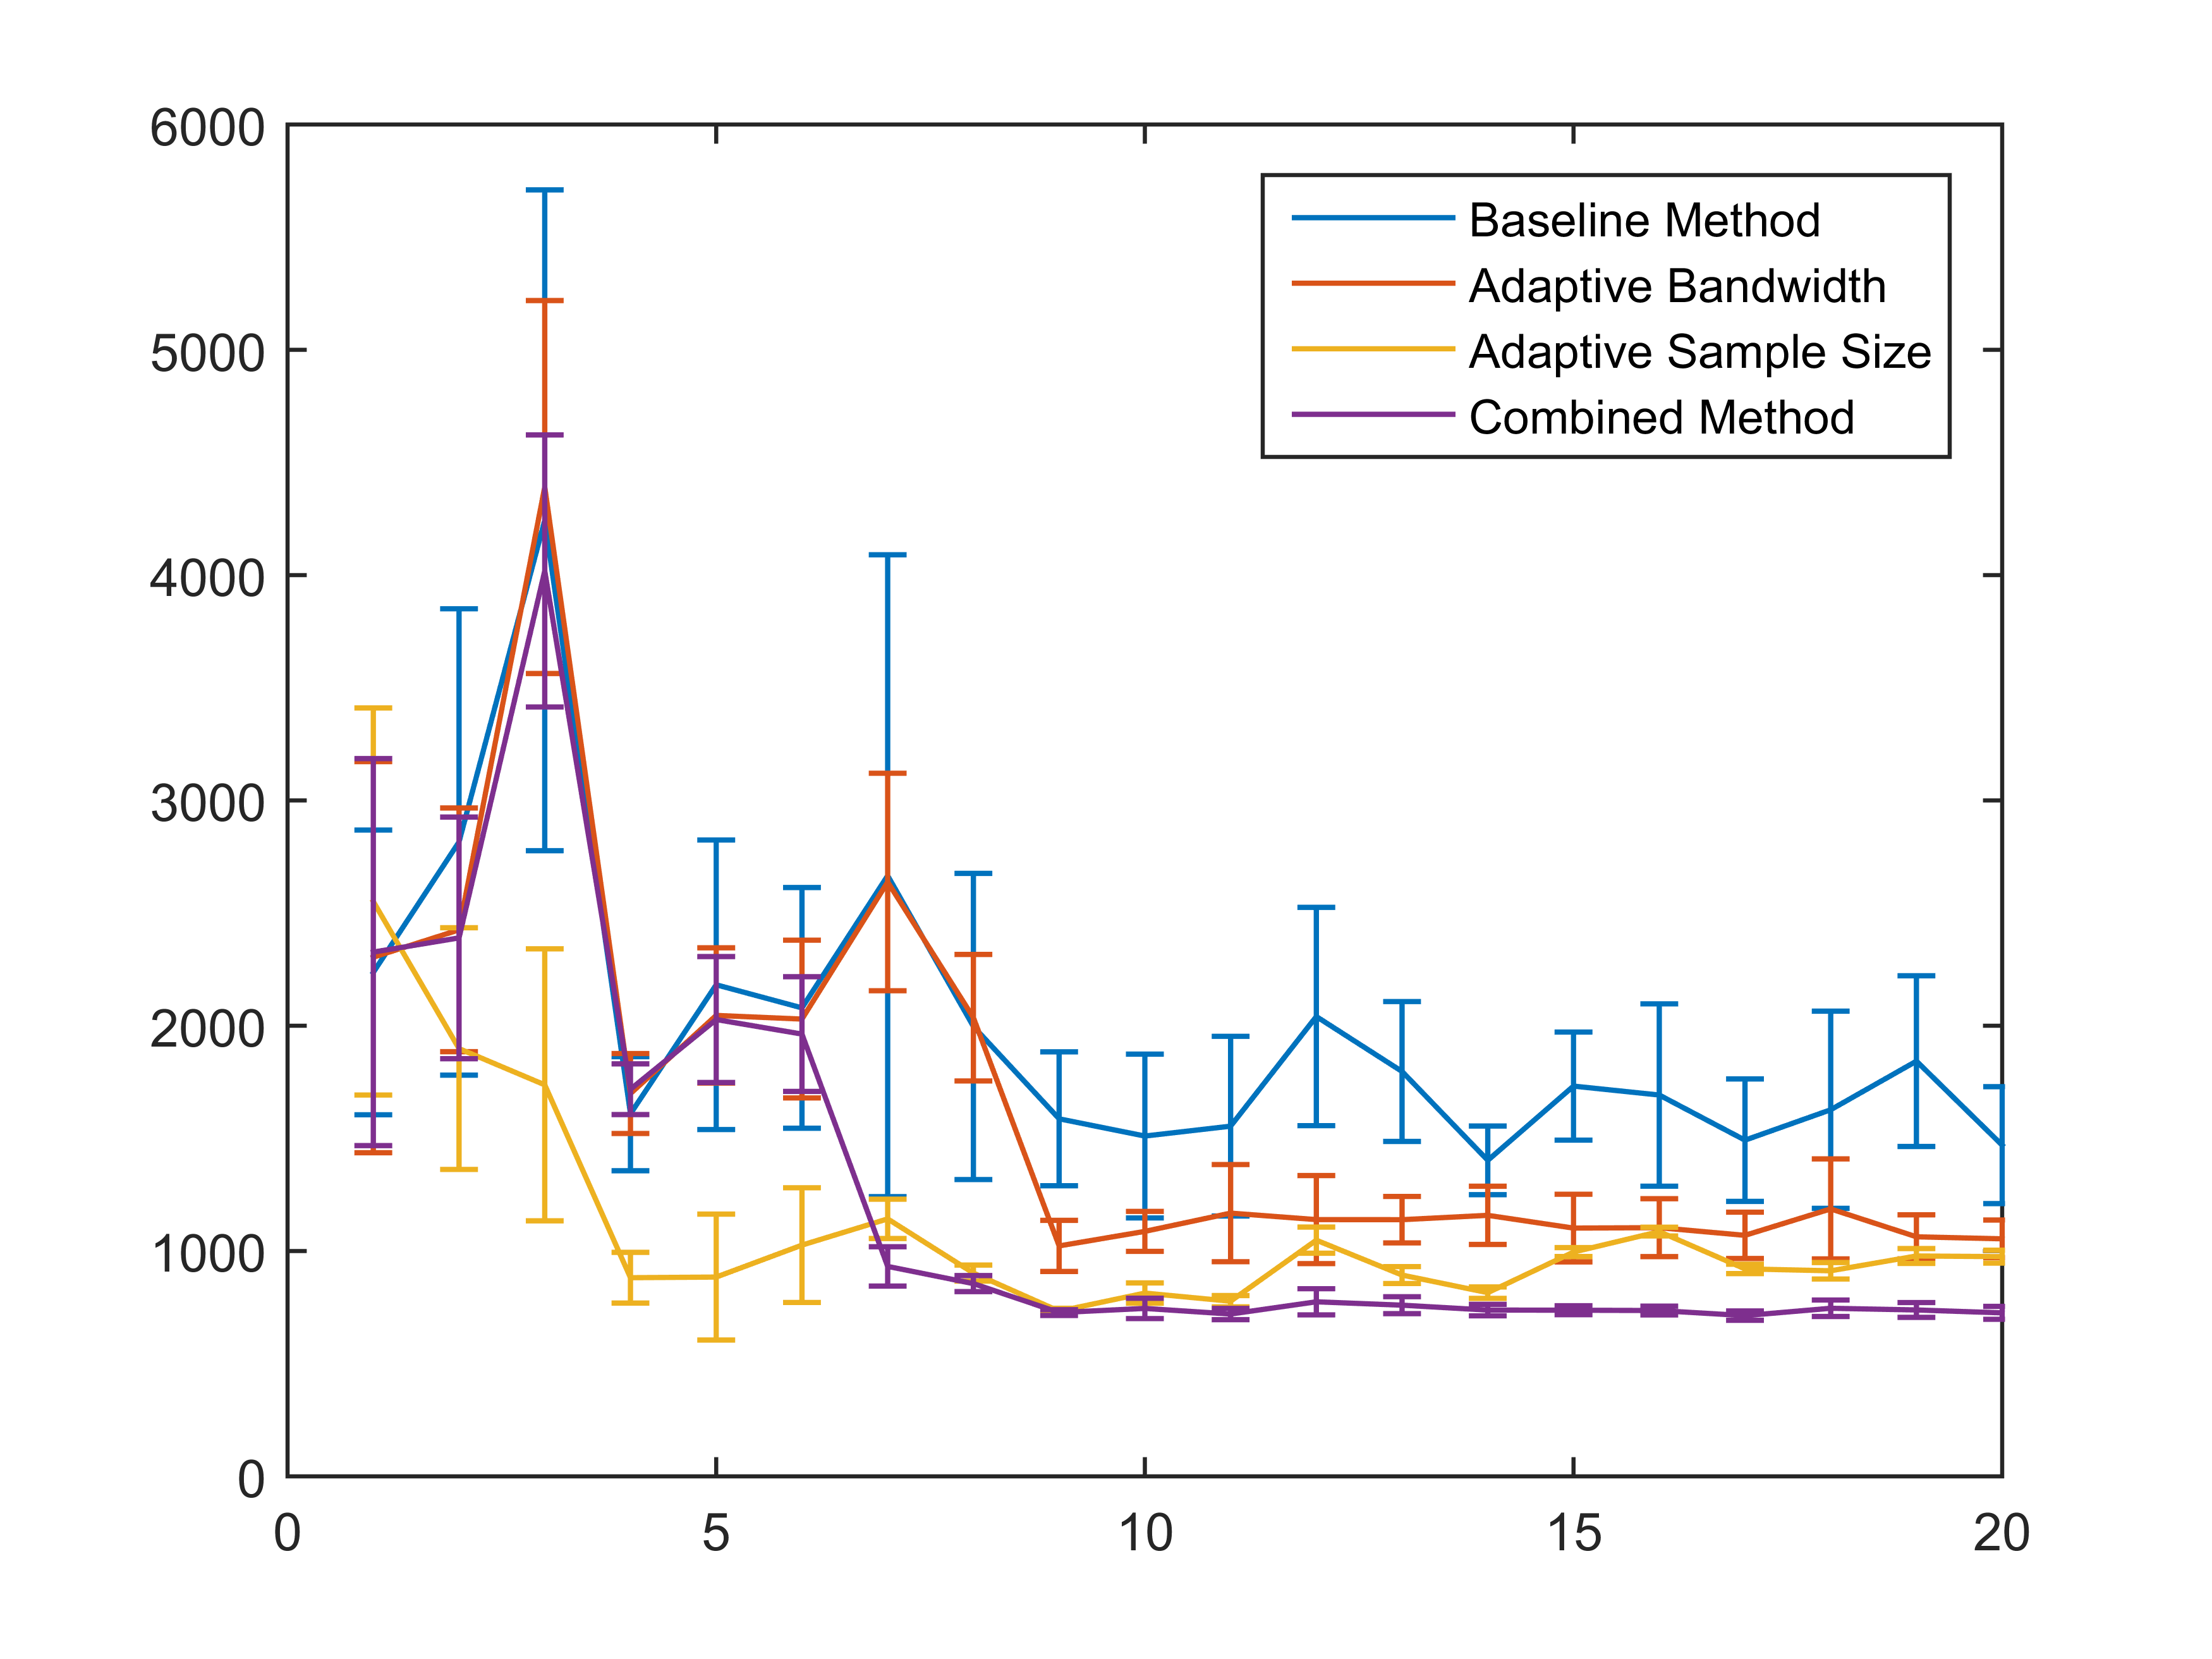
\includegraphics[width=.5\linewidth]{./Localization/time_method}};
  \node[left=of img, node distance=0cm, rotate=90, anchor=center,yshift=-1cm] 
       {Time for Particle Update (ms)};
  \node[below=of img, node distance=0cm, yshift=1.2cm] 
       {Measurement Number};

\end{tikzpicture}


\caption{Comparison of the time and accuracy of the particle filter update step when using Adaptive Bandwidth and Adaptive Sample Size}
\label{fig:FasterParticles}
\end{figure}


Suppose that the true distribution is given by a discrete multinomial distribution with $k$ different bins, it can be shown that with probability $1-\delta$, the KL-divergence is less than or equal to $\epsilon$ when the sample size $n$ is given by \cite{Fox2003}:

\begin{align}
   n &= \frac{1}{2\epsilon} \chi_{k-1, 1-\delta}^2 \\
   \label{eq:17}
   &\approx \frac{k-1}{2\epsilon} 
     \left( 1-\frac{2}{9(k-1)} + \sqrt{\frac{2}{9(k-1)} z_{1-\delta} } \ \right)^3
\end{align}
where $\chi_{k-1, 1-\delta}^2$ is the upper $1-\delta$ quantile of $\chi^2$-distribution with $k-1$ degrees of freedom, and $z_{1-\delta}$ is the upper $1-\delta$ quantile of the normal distribution.

%% Therefore, the number of particles $n$ can be adjusted according to the number $k$ of bins with support, as shown in Eq. \ref{eq:17}. The bins are implemented as a multidimensional grid with fixed size in the configuration space. During sampling, the number $k$ of occupied bins is counted simultaneously whenever the newly sampled state falls into an empty bin. The current sample size is counted and each increment of $k$ will result in an update of the desired sample size $n$. When the actual number of particles reaches the desired value or a predefined minimal limit, whichever is smaller, the sampling process finishes.

Therefore, the number of particles $n$ can be adjusted according to the number $k$ of bins with support, as shown in Eq. \ref{eq:9}. The bins are implemented as a multidimensional grid with fixed size in the configuration space. During sampling, the number $k$ of occupied bins is counted whenever the newly sampled state falls into an empty bin. The current sample size is counted and each increment of $k$ will result in an update of desired sample size $n$. When the actual number of particles reaches the desired value or a predefined maximal limit, whichever is smaller, the sampling process finishes.






Figure \ref{fig:FasterParticles} shows the comparison between the particle filters with different improvements that are mentioned above. 
The simulation uses a mesh model with 39444 triangles. 
The set of measurements used for each method is fixed and predefined. 
The baseline method represents the particle filter that only implements adaptive voxelization while using fixed kernel bandwidth $h=0.0035$ and fixed number of particles ($n=500$). 
Adaptive Bandwidth improves the convergence accuracy significantly compared to the baseline method, while Adaptive Sample Size generally leads to poorer convergence with faster speed. 
The combined method applies all of the improvements above. 
It can achieve both faster and more accurate convergence compared to the other methods.

%% \subsection{Modeling Part Uncertainty: Problems with the Standard Particle Filter} 

%% At each time step, the belief is a probability distribution of poses, approximated using a particle filter. 
%% This belief distribution is also used to plan measurements actions that maximize the expected information gain. 
%% The advantage of using a particle filter over other Bayes estimation methods, such as the original\cite{kalman1960new}, extended\cite{kalman1961new} or unscented\cite{julier1997new} Kalman filter, is that a particle filter can model multi-modal non-Gaussian distribution with a non-linear measurement model.


%% The belief of the state at time $t$ is dependent on the measurements: $bel(x_t) = p(x_t| z_1, \textellipsis, z_t, x_0)$. The measurement model follows a non-linear probabilistic function of the true state: $\measurement_t \sim p(\measurement_t|\state_{actual})$. 
%% As in all Bayesian filters, the belief $bel(x_{t+1})$ is calculated recursively as follows\footnote{The full update of a Bayesian filter also includes a process model.
%% The assumption of a fixed object yields the static process model and this simpler formulation} \cite{Thrun2000}:
%% \begin{align}
%% bel(x_{t+1}) \leftarrow \eta \ p(z_t|x_{t+1}) \  bel(x_t)
%% \end{align}
%% with $\eta$ as a normalization factor. Each new measurement value triggers an update to the belief $bel(x)$. 

%% \subsection{Rejection Sampling to Overcome Particle Starvation}
  
%% The traditional particle filter uses importance sampling to update particles \cite{Thrun2000}, where samples are drawn based on the process model and weighted by the observation. However, for precise measurements and higher dimensions, the chance that a particle is consistent with the measurement is extremely low, thus few of them will survive during the update \cite{Koval2013}. 
%% Alleviating this problem would require an exponential (in the dimension of the state) number of particles to maintain high enough particle density.

%% Instead, the approach used updates the particles using rejection sampling \cite{Saund2017}. At each update step $t$, the continuous prior belief is estimated using Gaussian Mixture Models by applying a Gaussian kernel to each particle, with the kernel covariance proportional to the covariance of the particle configurations. 
%% New samples $\particle[t+1][i]$ are then drawn directly from this estimated prior. 
%% Using rejection sampling, each sample is accepted with probability $p(z_t|\particle[t+1])$. 
%% Sampled configurations with the part boundary far from the measured contact location, and thus inconsistent with the measurement, will have a low probability of being accepted
%% %% This probability depends on the actual distance between the measurement and the object: if the object with pose $\particle[t]$ is sufficiently far away from the measurement, the sample will be rejected.

%% The computational cost of potentially rejecting many samples is offset by using a voxelized distance field \cite{Felzenszwalb2004}, where the distance between each voxel in 3D workspace and the object is precomputed. 
%% As the measurement $\measurement_t$ is described in the world frame, during the rejection sampling the measurement is transformed to the part frame before lookup in the distance field.
%% %% , as each sample represents a transformation relation $T(x_{t})$ from world frame to the part 
%% %% frame. 
%% The minimal unsigned distance $dist_u(\measurement_t,S)$ between each measurement $\measurement_t$ and the object $S(\particle[t+1])$ can be obtained directly\cite{Saund2017}: 
%% \begin{align}\label{eq:unsigned}
%% dist_u(M_t,S(\particle[t+1])) = D_f(T(\particle[t+1])^{-1}M_t)
%% \end{align}
%% \begin{align}\label{eq:signed}
%% dist(M_t,&S(\particle[t+1])) =\\
%%  &\left\{
%% \begin{array}{ll}
%% dist_u(M_t,S(\particle[t+1])) - r_p, & \text{if }M_t\notin S\\
%% -dist_u(M_t,S(\particle[t+1])) - r_p, & \text{otherwise}.
%% \end{array}
%% \right.
%% \end{align}  
%% where $D_f$ is the precomputed distance field, $r_p$ is the radius of the spherical tip of the touch probe. 
%% %% For 1D range finder, $r_p=0$.

%% New samples $x_t$ are accepted based on the signed distance $dist(M_t,S(x_t))$ between the object and the measurement on the object. Rejection sampling continues until a desired number of particles have been accepted for this update. 
%% These particles represent the updated belief $bel(x_t)$ of the pose. 


\section{Datum Based Particle Filter} \label{sec:datum}

The particle filter localization method presented above assumes that the object matches its CAD model exactly. 
However, this is usually not the case, due to tolerances in the manufacturing and assembly processes.
To handle manufacturing deviations, features on parts are not located with respect to the part frame, but with respect to datums, (edges, surfaces, and holes) on the actual ``as built'' part. Incorporating the notion of datums, and their relationships, adds complexity because the relationship between the datum and the CAD model contains uncertainty. Thus, measuring one section of the assembly provides only uncertain updates to other sections, dependent on the specified tolerances. 
The following formulation treats these as semi-rigid parts, where each complete part is composed of rigid \textit{sections}, coupled through a probabilistic distribution of transformations connecting the section frames.
%% The uncertainty in these internal transformation is usually small, but non-negligible, compared to the required accuracy of localization needed.
%% We will also refer to the datums and features as \textit{sections} of the part. 
%% The problem is that we want measurements on one section to update the position beliefs of other sections, and also that we want to determine the information gain on a section from measuring a different section.
The datum based particle filter is introduced to allow updates on the belief of all sections of a part using the prior distribution of coupling transformations, and a measurement on a single section.

\subsection{Datum Representation}

The formulation introduced here treats the overall part as composed of separate, known sections. 
The problem is to precisely localize some feature which cannot be measured \textit{directly} (e.g. a location to drill a hole) with respect to given datums (other sections). 
To localize the goal feature, certain datums must be localized in certain dimensions.
For instance, Figure \ref{fig:Overview:CAD} shows a hole feature referenced to the top and right edges datums of the part.
The true part configuration is shown in gray in \ref{fig:Overview:belief_top} and \ref{fig:Overview:belief_right}.
In this example, it is necessary to localize the top edge's vertical position and orientation, but not its in-page or horizontal position. 
Similarly, the right edge only must be localized horizontally.
% Belief Description of figure 1b
%% The issue is to maintain the transformation relations between sections so that when making one
%% measurement the distributions of all the associated sections are updated.

%% Instead of using a single CAD model for the whole object, separate mesh files are used for each section under the assumption that each physical section will match its CAD model precisely.

Two approaches are now introduced; the first explicitly represents
the joint probability distribution between the sections, and the second stores separate,
independent probability distributions for each section.
Figures \ref{fig:FullBelief} and \ref{fig:Overview} visualize the independent-state particle filter. The full-state particle filter produces similar images.
%% We continue to assume that the measurements will be made by point-based sensors.
 %% (touch probe or 1D laser range finder). 

The rest of this chapter uses the following notation.
$\particles[t][][k]$ is the set of N particles representing the belief of section $k$ at time step $t$.
Frequently $t$ is omitted when implicit.
Each particle is a configuration for a single section $\particles[][][k] = \{\particle[][j][k]\}_{j=1}^{N}$.
The omission of $k$ indicates all necessary particles to represent the belief of the part: $\particles = \{\particles[][][k]\}$ and $\particle = \{\particle[][][k]\}$.



\subsection{Geometric Relationships}

\begin{figure}
  \centering
  \begin{subfigure}[b]{.9\linewidth}
    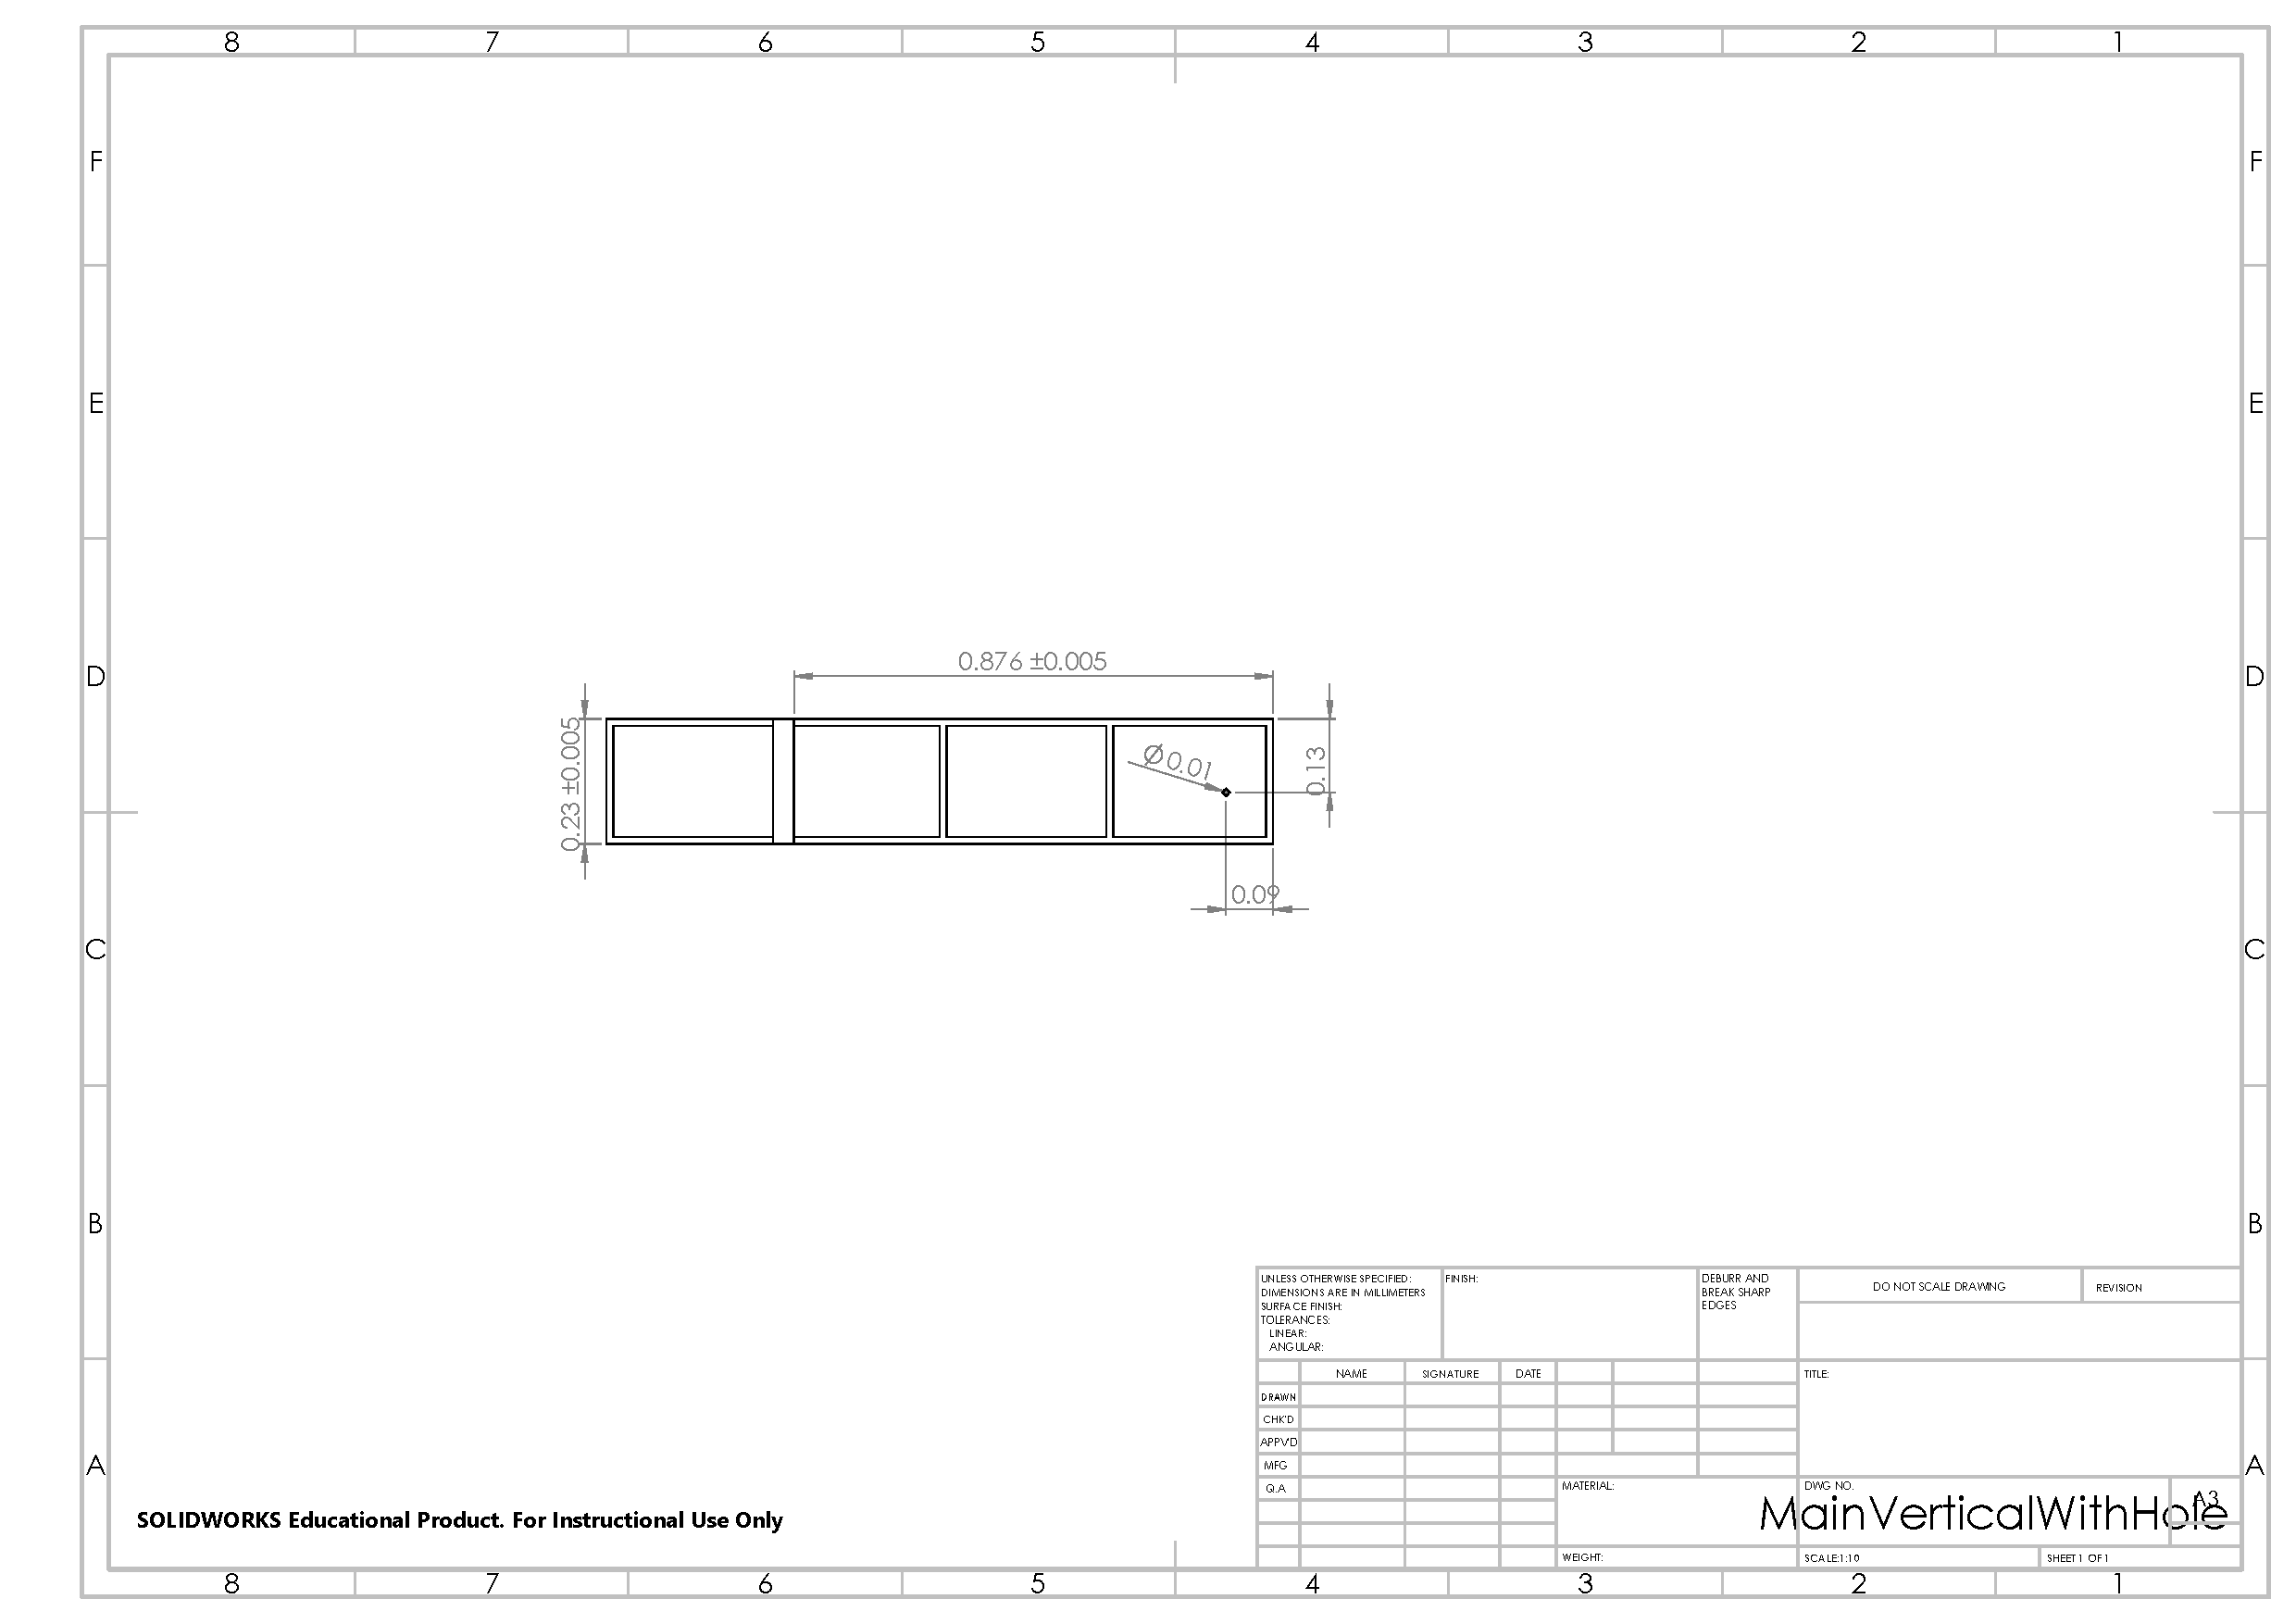
\includegraphics[width=\linewidth, clip, trim=4in 5in 6.5in 4.5in]{./Localization/MainVerticalWithHole}
    \caption{CAD}
    \label{fig:Overview:CAD}
  \end{subfigure}
  \hfill
  \begin{subfigure}[b]{.9\linewidth}
    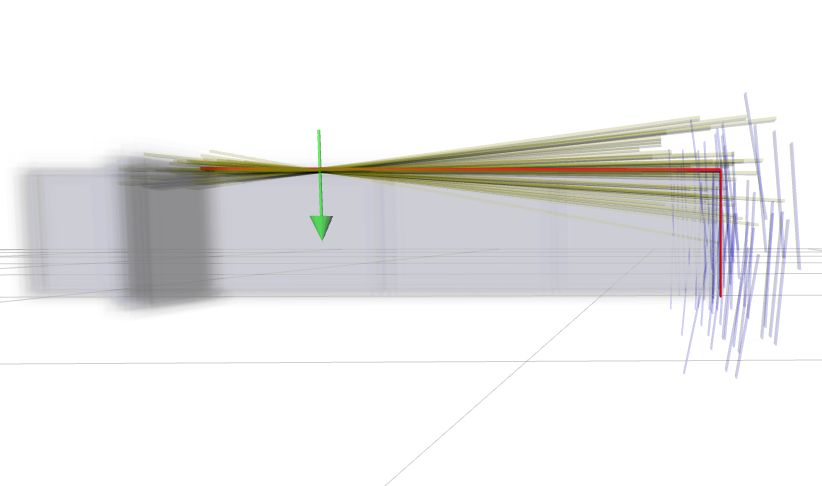
\includegraphics[width=\linewidth, clip, trim=0.1in 1.5in 0.3in 1.3in]{./Localization/final_result_4_2}
    \caption{Update from a measurement on the top datum}
    \label{fig:Overview:belief_top}
  \end{subfigure}
  \hfill
  \begin{subfigure}[b]{.9\linewidth}
    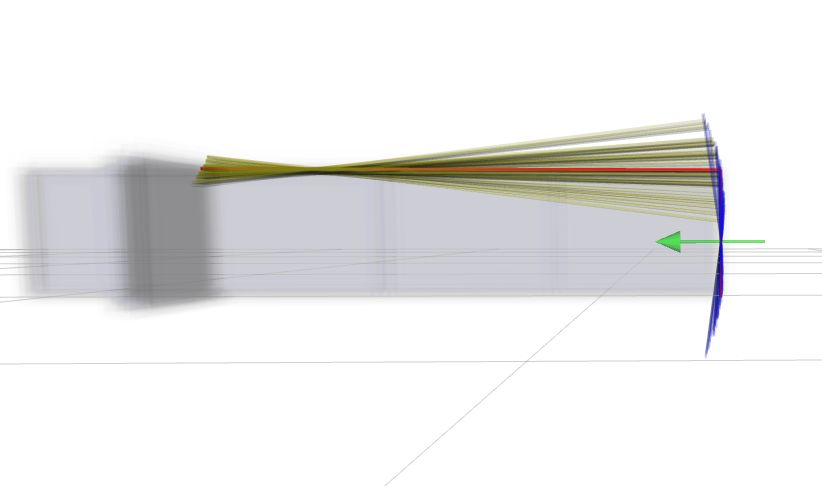
\includegraphics[width=\linewidth, clip, trim=0.04in 1.5in 0.35in 1.3in]{./Localization/final_result_4_3}
    \caption{Update from another measurement on the right datum}
    \label{fig:Overview:belief_right}
  \end{subfigure}
  \caption{
    Visualization of independent-state particle filter\\
\protect\subcap{fig:Overview:CAD}: Side view of the CAD drawing with dimensions (simplified for clarity). 
%The top and right edges serve as datums for the hole. 
This drawing indicates the nominal distance between the top and bottom edge is 0.23m, with a symmetric tolerance of 5mm.
This drawing also defines a hole with a 1cm diameter, and the top edge as its vertical datum and side edge as its horizontal datum.\\ 
\protect\subcap{fig:Overview:belief_top}: The beliefs of the top (green) and right (blue) edges of the part are shown. 
The true part location is shown in gray. 
The measurement (arrow) on the top section partially localized the top edge.
For clarity in the image, the belief of the other sections are not shown, and only 50 of the 500 particles are shown.\\
\protect\subcap{fig:Overview:belief_right}: 
A following measurement (arrow) on the right edge further localizes the part. 
This measurement provides information on the right edge directly, and the top edge indirectly.
}
  \label{fig:Overview}
\end{figure}

Geometric relationships are defined between two or more part sections. The existence of the tolerance introduces uncertainty to these relationships, which are modeled as a distribution of transformations in the configuration space between the pose of each section. 
More generally, the conditional probability $p(\particle[t][][k]|\mathbf{\particle[t]})$ represents the belief of the pose of section $k$ given the poses of the other sections.
%% $\mathbf{x_t}=\{\particle[t][][j]\}_{j \in J}$. 
%% The joint probability then becomes $bel(x^i_t, \mathbf{x_t}) = p(x^i_t|\mathbf{x_t})p(\mathbf{x_t})$. 


%
%\begin{figure}
%	\centering
%	\begin{tikzpicture}
%	\tikzstyle{main}=[circle, minimum size = 8mm, thick, draw =black!80, node distance = 6mm and 14mm]
%	\tikzstyle{connect}=[-latex, thick]
%	\tikzstyle{box}=[rectangle, draw=black!100]
%	\node[main, fill = white!100] (A) [label=center:\normalsize $A$] {};
%	\node[main] (C) [right=of A,label=center:\normalsize $C$] {};
%	\node[main] (B) [above=of C,label=center:\normalsize $B$] {};
%	\node[main] (D) [below=of C,label=center:\normalsize $D$] {};
%	\node[main, fill = black!10] (E) [right=of D,label=center:\normalsize $E$] {};
%	\node[main] (F) [right=of C,label=center:\normalsize $F$] {};
%	\path (A) edge [connect] (B)
%	(A) edge [connect] (C)
%	(A) edge [connect] (D)
%	(B) edge [connect] (F)
%	(C) edge [connect] (F)
%	(C) edge [connect] (E)
%	(D) edge [connect] (E)
%	(E) edge [connect] (F);
%	
%	\end{tikzpicture}
%	\caption{}
%	\label{Graphical Model}
%\end{figure}


A measurement is made on a single section at each step by a touch probe.
Let the measurement on the section $k$ at step $t$ be $\maction^k_t$, then the posterior of section $k$ is $p(\particle[t][][k]|\mathbf{\particle[t]}, \measurementSet^k_t)$. 
In the following algorithms, the section that a measurement contacts is known.
This assumption is reasonable if the uncertainty of the prior belief is small compared to the physical size of each section, and measurement are not chosen on the boundary between sections.
If this assumption does not hold, localization can be performed for the whole object using the methods of section \ref{sec:rigid_body} to get better estimate, before considering the object as a combination of coupled sections.

%% The conditionals are only a prior estimate of the geometry transformations. During updates, both the transformations between sections and the pose of sections itself need to be refined based on the measurement.

\subsection{Full-State Representation} \label{sec:full state}

\begin{figure}
	\centering
	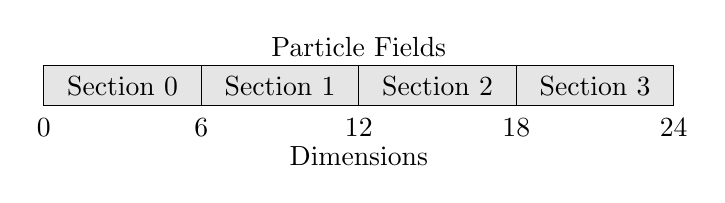
\begin{tikzpicture}
	\draw (0,0) -- (8,0);
	\draw (0,0) -- (0,0.5);
	\draw (2,0) -- (2,0.5);
	\draw (4,0) -- (4,0.5);
	\draw (6,0) -- (6,0.5);
	\draw (8,0) -- (8,0.5);
	\draw [fill=black!10] (0,0) rectangle (2,0.5);
	\draw [fill=black!10] (2,0) rectangle (4,0.5);
	\draw [fill=black!10] (4,0) rectangle (6,0.5);
	\draw [fill=black!10] (6,0) rectangle (8,0.5);
	\node[align=left, below] at (0,-.05) {0};
	\node[align=left, below] at (2,-.05) {6};
	\node[align=left, below] at (4,-.05) {12};
	\node[align=left, below] at (6,-.05) {18};
	\node[align=left, below] at (8,-.05) {24};
	\node[align=center, below] at (4,-.4) {Dimensions};
	\node[align=center, above] at (1,0) {Section 0};
	\node[align=center, above] at (3,0) {Section 1};
	\node[align=center, above] at (5,0) {Section 2};
	\node[align=center, above] at (7,0) {Section 3};
	\node[align=center, above] at (4,.5) {Particle Fields};	
	\end{tikzpicture}
	\caption{A 24-dimensional particle for object with 4 sections}
	\label{fig:full-state}
\end{figure}

The first method presented maintains the full joint probability distribution between sections using a single set of full-state particles: $\particles[t] = \{\particle[t][j]\}$. 
%% A Bayesian network is defined where the nodes are sections and the edges are the transformation relationships.
%% The transformation between sections are defined in a graph, such that sections 
%% Defining transformations of the sections in a graph is natural. 
%% The sections which are related by the geometry constraints can be modeled as nodes in the graph, while the constraints serve as edges. 
%% An example is Bayesian network, where the geometry relations between a section and its referenced datum are represented by directed edges. 
%% The advantage for this representation is that we can restore the full joint distribution using fewer edges within Markov blanket. 
%% However, for non-parametric continuous distribution, it is difficult to apply belief propagation approaches to update the whole graph given an observation on a section. 
%% Instead, for the object in 3D workspace with $n$ sections being tracked, we explicitly maintain a full $6n$-dimensional state space. 
Thus, each particle represents a combination of the poses of all of the sections (see Fig. \ref{fig:full-state}), which is drawn from the prior joint distribution $bel(\particle[0])$.

Instead of applying a Gaussian kernel in 6D configuration space as done in section \ref{sec:rigid_body}, the continuous prior is estimated by Gaussian Mixtures in the full $6n$-dimensional configuration space, with the kernel covariance proportional to the covariance of the sampled states. This is achieved by applying kernel density estimation techniques. One popular method for the bandwidth selection is the Silverman's rule-of-thumb estimator\cite{Silverman1986}. Other techniques are discussed in more detail in \cite{sheather2004density}.


Although it seems at first that the high dimensional state space will require a prohibitively huge number of particles to approximate the true distribution, in practice, this has been found to not the case. 
Largely, this is due to the small internal tolerances compared to the uncertainty of the pose of the object as a whole, so particles tend to cluster in a small subset of the full state space. 
Note that if there were no uncertainty in the transformation between sections, then the system reduces to a single 6 dimensional state space.
In addition, the Gaussian kernel applied to the particles is capable of creating broad beliefs in specific dimensions\cite{Saund2017}, thus this particle filter is able to model the mixture of precisely localized, and poorly localized dimensions. 
Finally, the sample acceptance probability, $p(z_t|\particle[t])$, depends only on the 6 dimensional subspace corresponding to the pose of the section being touched, and although only a thin manifold is accepted with high probability, the particle starvation challenge is no worse than previously addressed in \ref{sec:rigid_body}.
%% We suspect there is an approximate lower dimensional structure which this particle filter captures.


\begin{algorithm}[t]
  \caption{Full-State Particle Filter}\label{alg:full state}
  \begin{algorithmic}[1]
    \Require{number of particles $N$ and number of sections $n$ }
    \Require{particles $\mathbf{\particles[t]}$}
    \Require{observation $\measurement^i_t$}
    \Require{meshes $S=\{S_k\}^n_{k=1}$}
    \Ensure{particles $\mathbf{\particles[t+1]}=\{\mathbf{\particle[t+1][j]}\}^N_{j = 1}$}
    \State build distance field $D_f(p)$
    \State $j \gets \mathbf{1}$
    \While{$j\le N$}
    \State $\mathbf{x}\sim p(\particle|\mathbf{\particles[t]})$ \Comment $\particle = \{\particle[][][k]\}^n_{k=1}$
    \State $dist \gets D_f(T(\particle[][][i])^{-1}\measurement^i_t)$
    \If{$dist \le \xi$}
    \State $\particle[t+1][j]\gets \particle$
    \State $j \gets j+1$
    \EndIf
    \EndWhile
  \end{algorithmic}
\end{algorithm}

At any time step $t$ the belief of the state $bel(\mathbf{\particle[t]}) = p(\mathbf{\particle[t]}| Z_t, \particle[0])$, and $\particle[t][][k]$ is the portion of $\particle[t]$ representing the pose of section $k$. 
%% As for rigid part localization, the belief is estimated by a single set of particles and updated using rejection sampling. 
During rejection sampling, new full-state samples $\particle[t+1]$ are drawn from the estimated $\hat{bel}(\mathbf{x_t})$ directly. 
The probability of accepting a sample is based on the measurement $M^k_t$ on section $k$, and is computed by extracting the 6D pose $\particle[t+1][][k]$ from each full-state sample $\particle[t+1]$. Equation \ref{eq:unsigned} and \ref{eq:signed} are then used for the rejection sampling, except that the transform from the extracted $\particle[t+1][][k]$ is used to transform the measurement. 
If $dist(M^k_t,S_k(\particle[t+1][][k]))$ is sufficiently large, this full-state sample $\mathbf{x_{t+1}}$ is rejected, otherwise accepted. 
Note that the full-state sample $\mathbf{x_{t+1}}$ is accepted based on $p(M^k_t|\particle[t+1][][k])$, and the CAD model used for distance field $k$ is the mesh for that particular section, $S_k$ (shown in Algorithm \ref{alg:full state}). For simplicity, the pseudo-code does not include the adaptively adjusted sample size based on KL-divergence\cite{Saund2017}\cite{Fox2003}. 

%% Each measurement made on a section updates the estimate of the full joint distribution for all sections based on how well the estimate is consistent with that measurement.
%% This updates all sections for one single measurement based on the transformation information in the prior belief without explicitly implementing the transformation.



\subsection{Independent-State Representation} \label{sec:independent state}

\begin{algorithm}[t]
  \caption{Independent-State Particle Filter}\label{alg:indep}
  \begin{algorithmic}[1]
    \Require{number of particles $N$ and number of sections $n$ }
    \Require{sets of particles $\mathbf{\particles[t]}=\{\particles[t][][k]\}^n_{k = 1}$}
    \Require{observation $\measurement^i_t$}
    \Require{meshes $S=\{S_k\}^n_{k=1}$, }
    \Require{transformations $\{p(T^k_i)\}^n_{k=1}$}
    \Ensure{particles $\mathbf{\particles[t+1]}=\{\particles[t+1][][k]\}^n_{k = 1}=\{\particle[t+1][j][k]\}$}
    \State build distance field $D_f(p)$ for section $S_i$
    \For{$k=1, ..., n$}
    \State $j \gets 1$
    \While{$j\le N$}
    \State $\particle\sim p(\particle[][][k]|\particles[t][][k])$
    \State $T^k_i\sim p(T^k_i)$ 
    \State $\sampled \particle\gets T^k_i\times \particle$ 
    \State $dist \gets D_f(T(\sampled x)^{-1}M^i_t)$
    \If{$dist \le \xi$}
    \State $\particle[t][j][k]\gets \particle$
    \State $j \gets j+1$
    \EndIf
    \EndWhile
    \EndFor
  \end{algorithmic}
\end{algorithm}

The first approach described above tracks the updates of both the pose of each datum and the their transformations by maintaining a full-state representation of the distribution.
An alternative is to maintain the probability distribution for each section separately.
Instead of using a full high-dimensional particle filter for the full object, individual 6-dimensional particle filters are used for each individual section under the approximation that the belief over transformations between sections are fixed and independent.
While this loses information compared with the full joint belief, in practice this loss is acceptable.

As in the rigid body particle filter described in \ref{sec:rigid_body}, a sample in the particle filter for section $k$ represents a $SE(3)$ pose of the geometry of section $k$. 
The transformation information between different sections are defined explicitly. 
The prior belief on the transformation from section $k$ to section $j$ is $bel(T^j_k)$, which is a distribution over $SE(3)$ transformations. 
A measurement on a single section updates all individual particle filters related through a defined transformation distribution.
Given a measurement $M^k$ on the section $k$, the updated belief becomes $p(\particle[t+1][][j]|T^j_k,M^k)$ for a related section $j$.

The update to the belief $bel(\particle[t][][k])$ given a measurement performed on section $k$ itself is identical to the particle filter update for the rigid object. 
Since $T^k_k$ is the identity with probability 1, the updated belief can be written as:
\begin{align}
bel(\particle[][][k]) &= p(\particle[][][k]|T^k_k,M^k) =p(\particle[][][k]|M^k)
\end{align}
For a section $j$ that references section $k$ ($k \neq j$), each new sample $\particle[t+1][][j]$ is drawn from the prior of its corresponding particle filter $j$. 
$\particle[t+1][][j]$ is then transformed from the frame of section $j$ to the frame of section $k$: 
\begin{align}
\sampled{x}^k = {^iT^k_j} \times \particle[][][j]
\end{align}
where $ ^iT^k_j \sim bel(T^k_j)$ is a sampled transformation from the distribution $bel(T^k_j)$.
As the measurement was performed on section $k$, the geometry of section $k$ is used rather than $j$ when computing the consistency with the measurement. 
%% Relatively in the frame of section $i$, the agreement between the measurement $M_t$ and the geometry $S_i(\particle[][j])$ of the section $i$ is computed. 
The sampled particle is accepted with probability $p(M_t|\sampled{x}^k)$. 
The above process is repeated until the desired number of particles have been accepted (shown in Algorithm \ref{alg:indep}).




%%%%%%%%%%%%%%%%%%%%%%%%%%%%%%%%%%%%%%%%%%%%%%%%%%%%%%%%%%%%%
\section{Predicting Effective Measurement Actions} \label{sec:information gain}
Performing measurements is expensive, so it is important to choose the measurement action that provides the most \textit{information gain} on the goal feature. 
Each action is treated as a probabilistic decision over a set of particles approximating the belief of the goal feature.
This is an approximation for the information gain for the underlying, continuous belief distribution.
The best measurement may not be on the goal feature, and it may be impossible to even measure the goal feature directly.
This formulation predicts the information gain on the goal feature for both a measurement directly on the goal feature, or indirectly for a measurement on datums or other sections of the part.

\begin{figure*}
    \hfill
    \begin{subfigure}[b]{0.2\linewidth}
        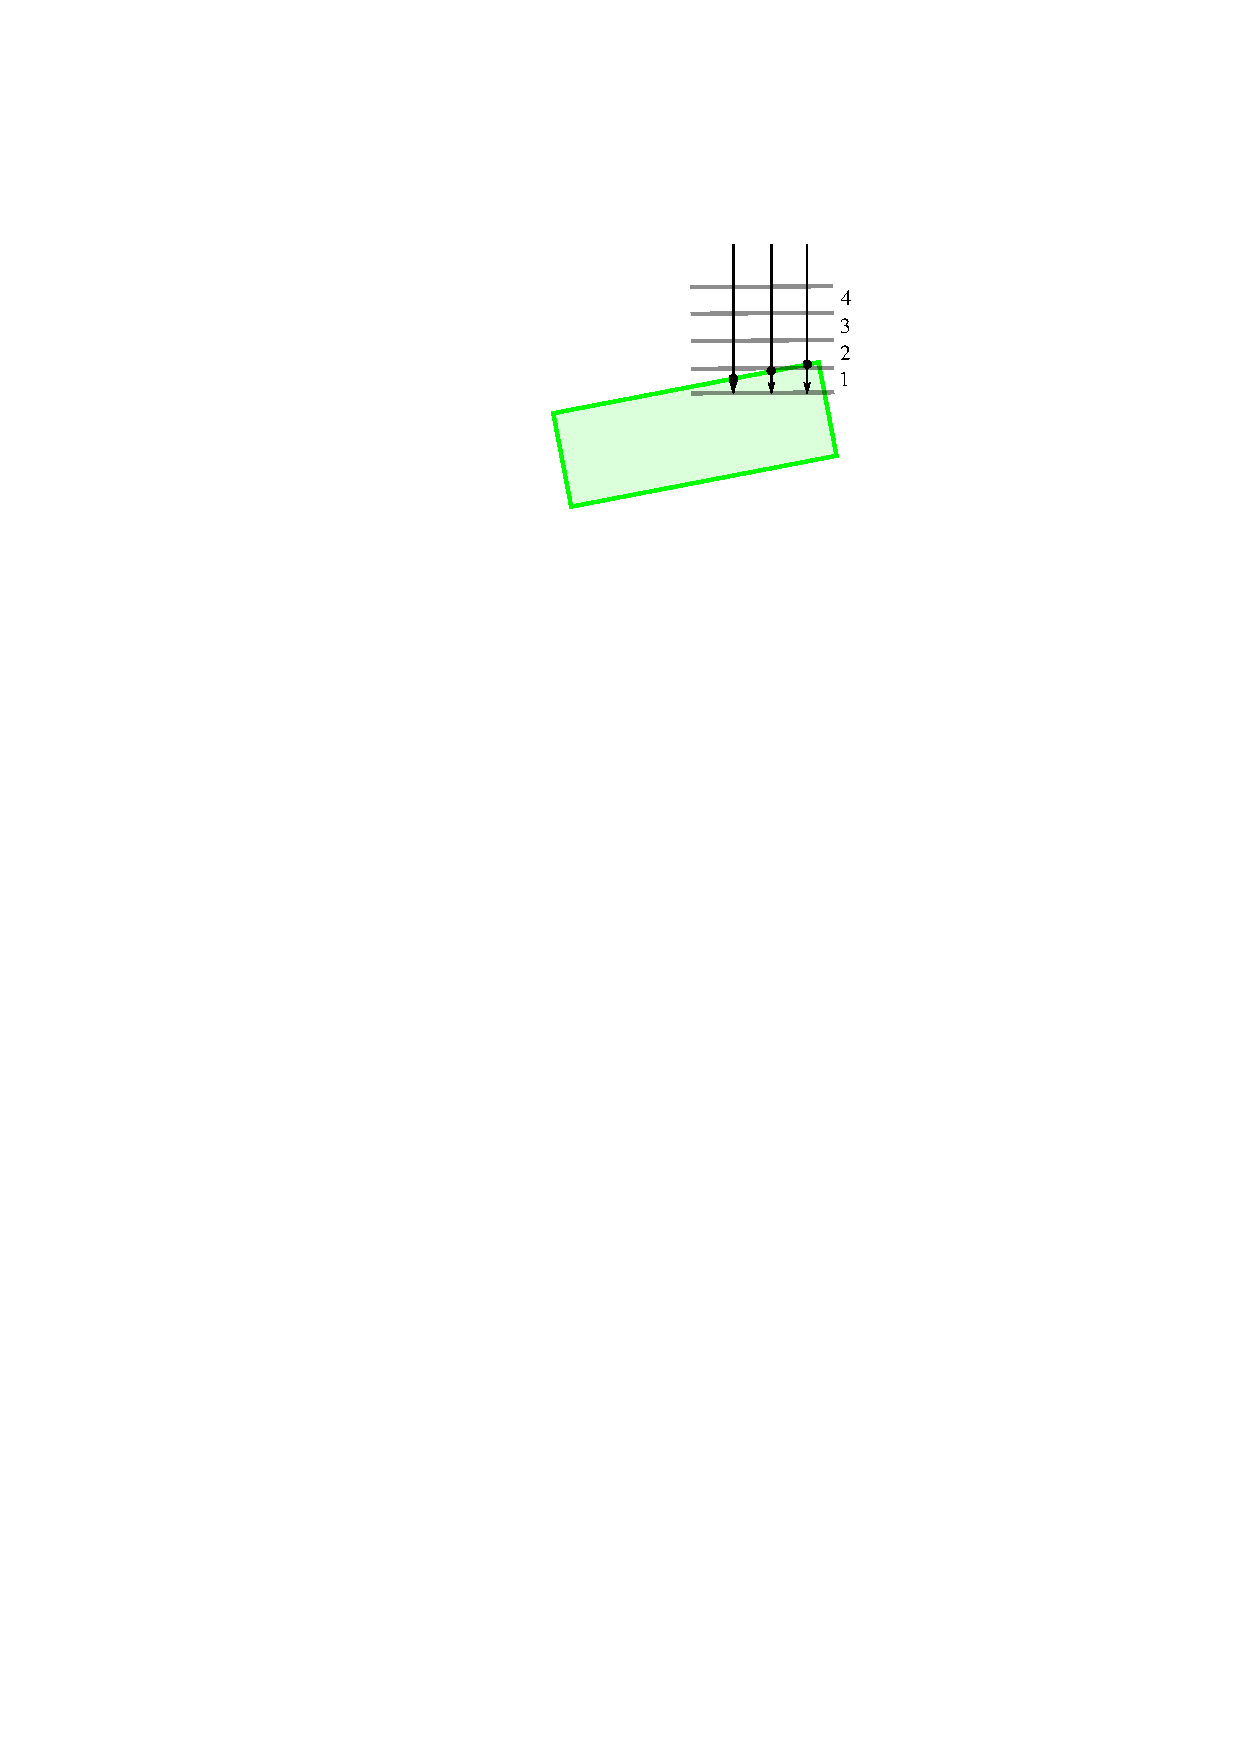
\includegraphics[width=\textwidth, clip, trim=4.2in 8.4in 2.5in 1.7in]{./Localization/bins_p1}
        \caption{Part in configuration: particle 1}
        \label{bins:p1}
    \end{subfigure}
    \hfill
    \begin{subfigure}[b]{0.2\linewidth}
        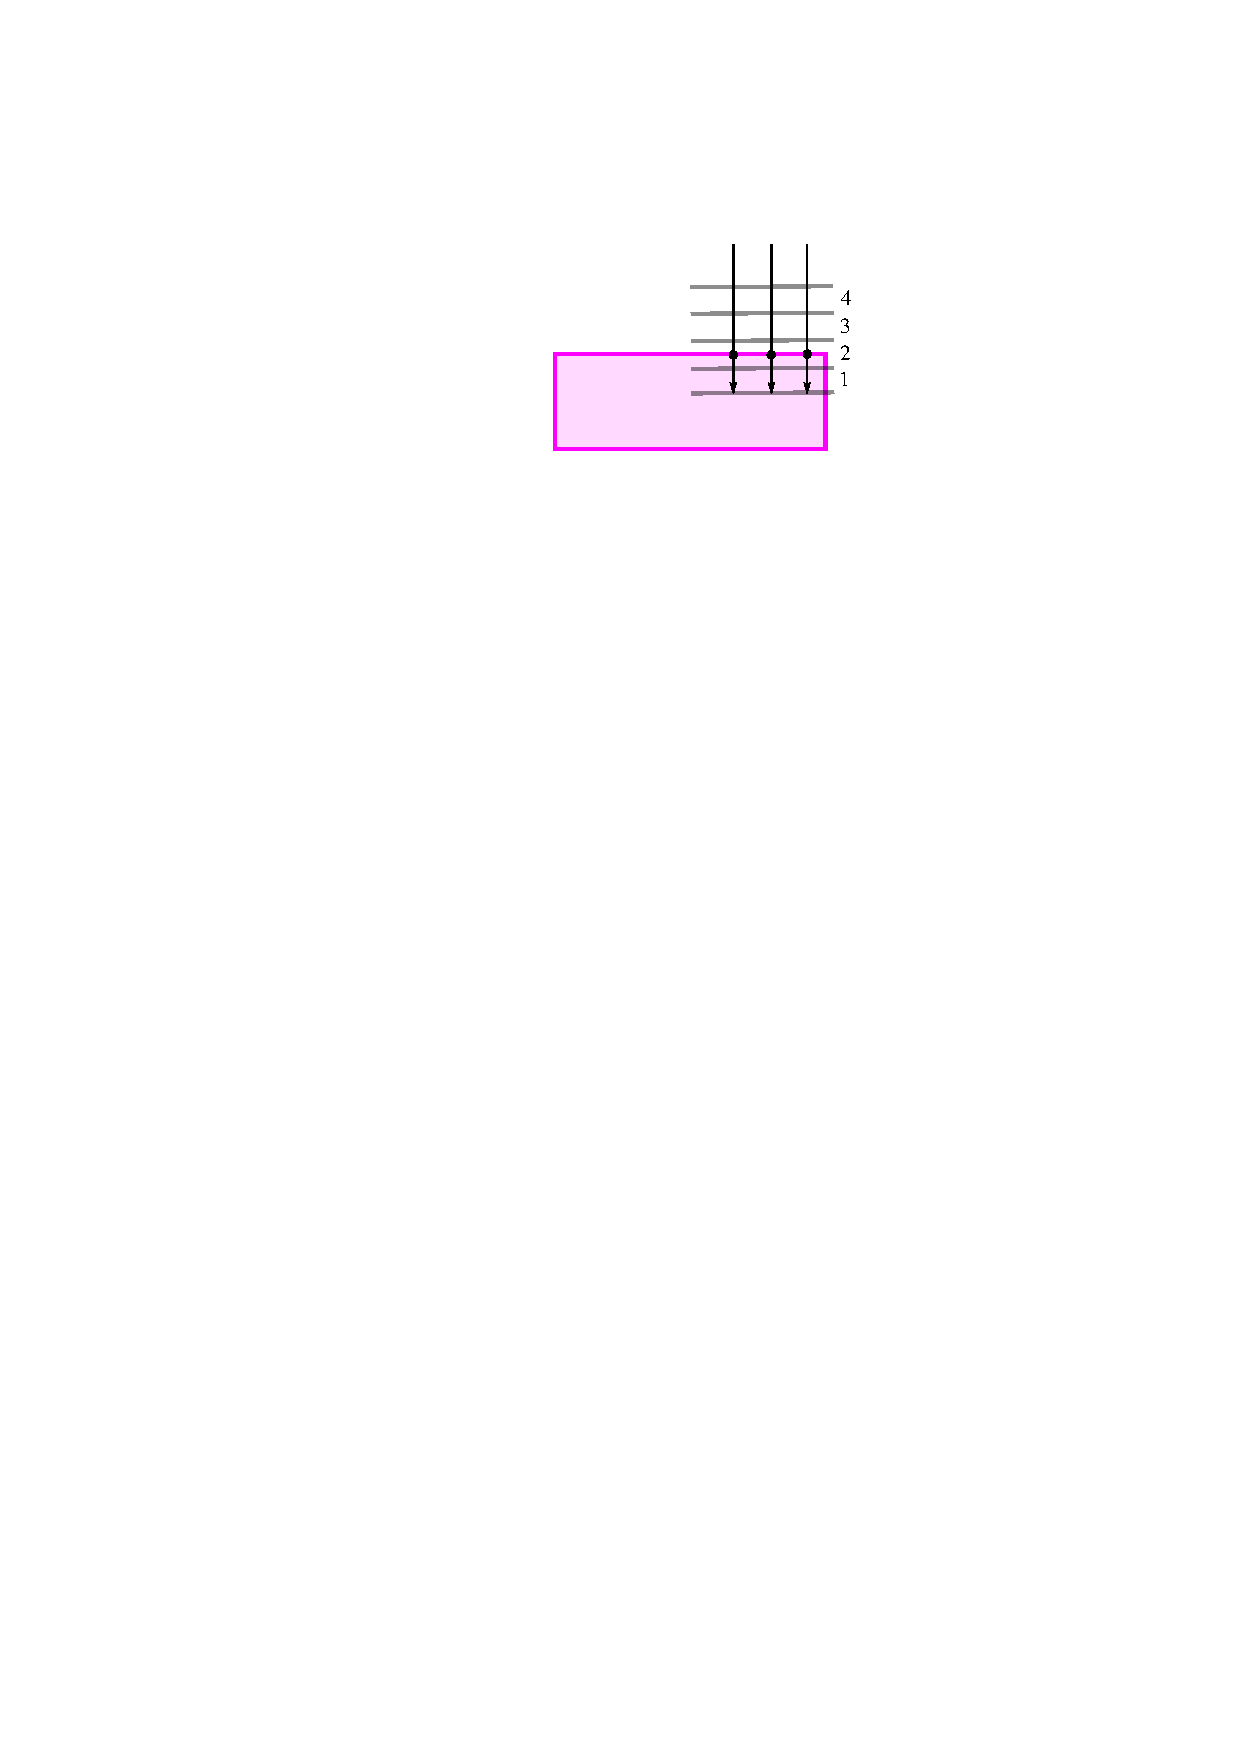
\includegraphics[width=\textwidth, clip, trim=4.2in 8.4in 2.5in 1.7in]{./Localization/bins_p2}
        \caption{Part in configuration: particle 2}
        \label{bins:p2}
    \end{subfigure}
    \hfill
    \begin{subfigure}[b]{0.2\linewidth}
        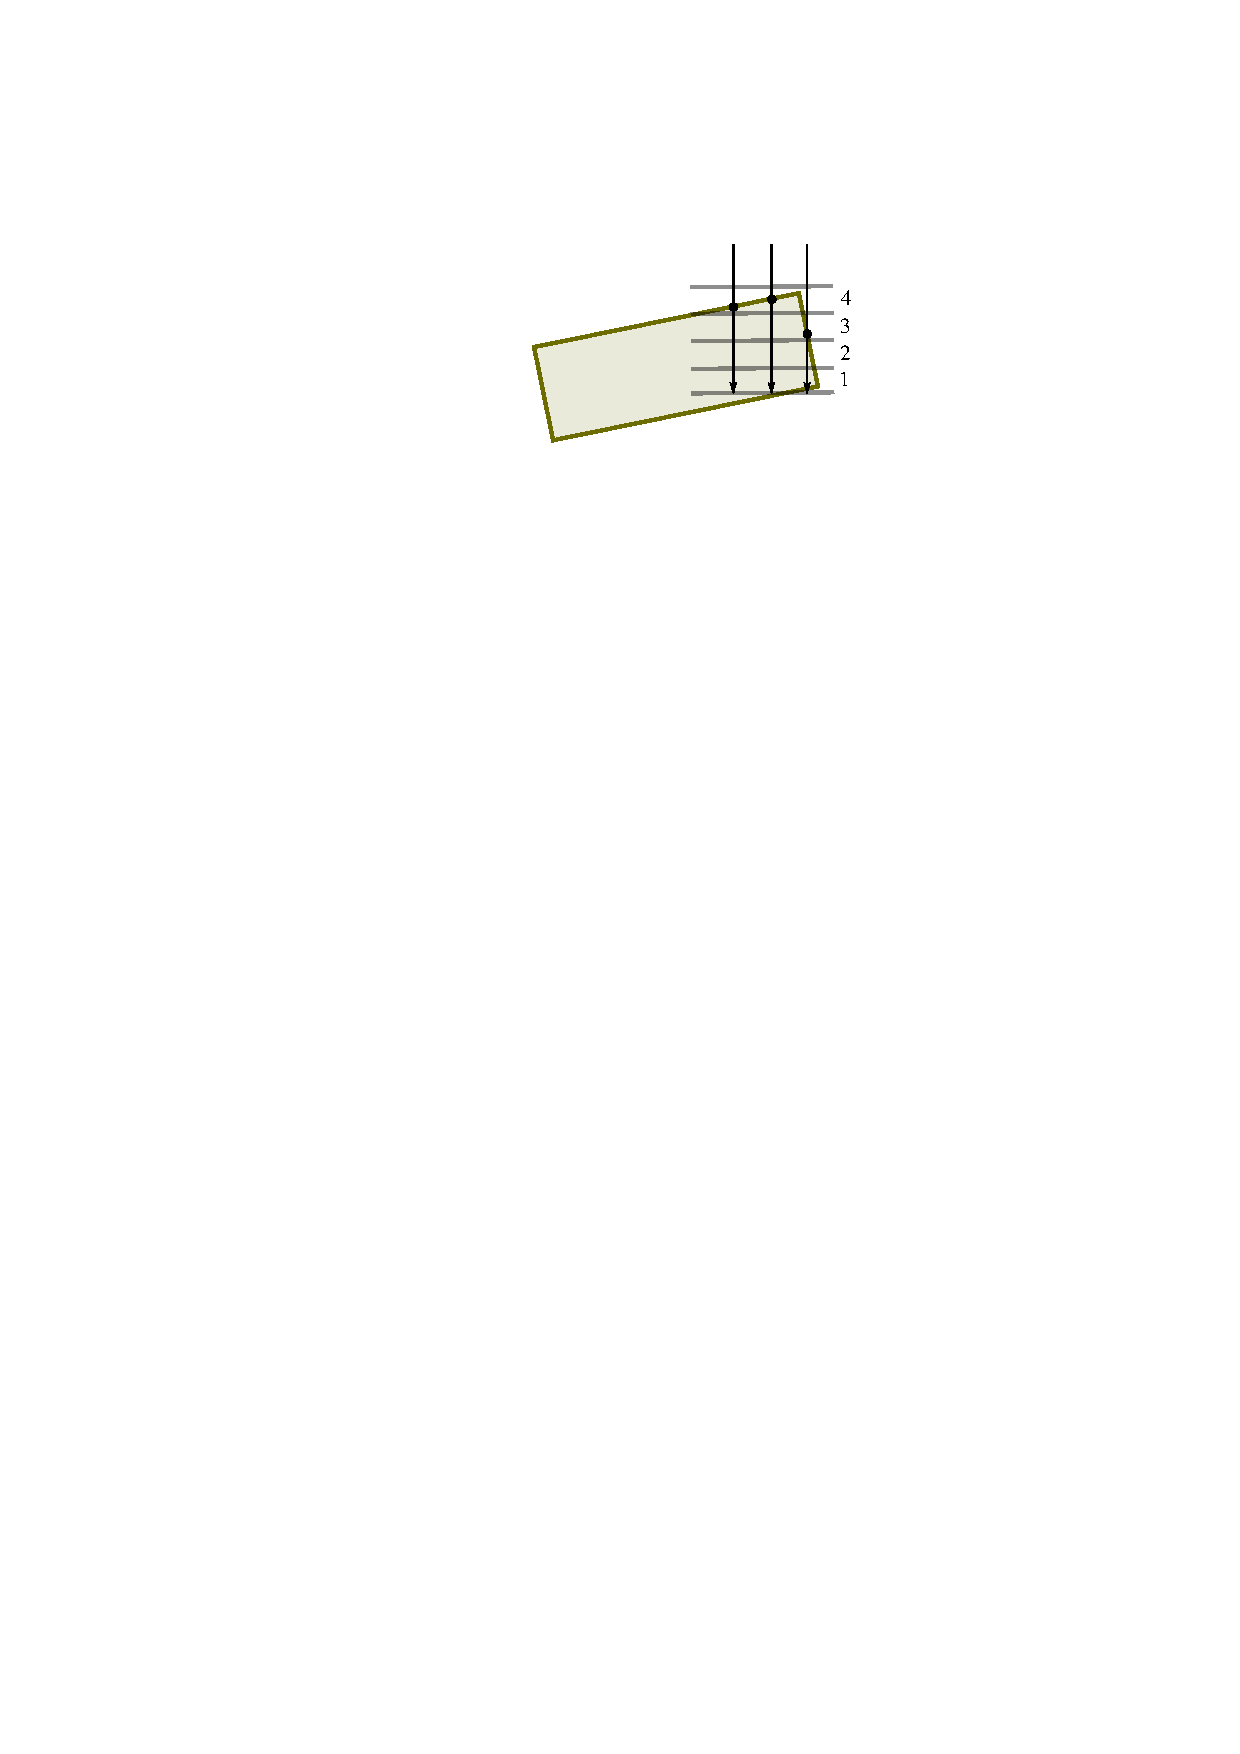
\includegraphics[width=\textwidth, clip, trim=4.2in 8.4in 2.5in 1.7in]{./Localization/bins_p3}
        \caption{Part in configuration: particle 3}
        \label{bins:p3}
    \end{subfigure}
    \hfill
    \begin{subfigure}[b]{0.38\linewidth}
        \includegraphics[width=\linewidth, clip, trim=1.2in 7in 4.1in 3.7in]{./Localization/bins_sorted}
        \label{figure:bins}
        \caption{Binned Measurements}
    \end{subfigure}
    \hspace*{\fill}
\caption{Binning of potential measurement on particles for use in calculating information gain. The three arrows represent the nominal measurement action $\maction$ with simulated deviation $\delta_j$. The horizontal lines divide the measurement values into the numbered bins.}
%% \caption{Heat maps showing information gain of vertical measurements during the localization process.
%% The intensity of every pixel is the normalized expected information gain of a measurement passing through the pixel orthogonal to the image.
%% Initially \subcap{heat:first} probing into the page is likely to miss the part, providing little information.
%% The first measurement reduced the uncertainty such that probing in this direction will more likely contact the part and provide information \subcap{heat:second}.
%% Repeating another measurement in the same place would not provide much information. 
%% \subcap{heat:third}
%% }
\label{fig:bins}
\end{figure*}



\subsection{Information Gain} \label{subsec:IG}
Given $\particles[][][G]$, a set of particles representing the belief of the goal feature, 
the \textit{information gain} from a measurement action $\maction$ is defined as the expected reduction of entropy.
\begin{align}
IG(\particles[][][G]|\maction) = H(\particles[][][G]) - H(\particles[][][G]|\maction)
\end{align}

$H(\particles[][][G])$ is the entropy of the particles and $H(\particles[][][G]|\maction)$ is the entropy of the particles conditioned on the measurement action.

The entropy of a discrete distribution of states depends only on the probabilities of each state occurring. 
\begin{align}
    H(\particles[][][G]) &= -\sum_i {w_i  \log w_i} 
\end{align}
where $w_i$ is the weight of particle $i$.
%% Note that the entropy does not depend on the location of the particles in the 6D pose space, and that a set of particles spread out can have the same entropy as a tightly packed set. 
%% This counter-intuitive definition is due to only considering the entropy of the discrete distribution of particles where every particle is distinct from every other particle, and ignoring continuous belief which the particles represent.

To calculate the conditional entropy, $H(\particles[][][G]|\maction)$, the measurement action $\maction$ is simulated on the part distribution. Performing a measurement action yields a continuous distribution of measurement value. $\totalWeight$ samples are drawn from this distribution for each particle:
\begin{align}
  \measurement_{i,j} = Simulate(\{\maction + \delta_j\}, \particles[][i][G]) + \eta_j \label{Eq:Simulate}\\
  j\in \{1, 2, \textellipsis, \totalWeight\}\\
  i\in \{1, 2, \textellipsis, N\}
\end{align}
where $\delta_j$ is the deviation from the nominal measurement action, $Simulate$ computes the value for a measurement action applied to the part in a specific configuration, and with $\eta_j$ as measurement noise.


\subsubsection{Measurement Simulation}


To predict the measurement value obtained from a measurement action: $p(m_j)$, the measurement uncertainty is again approximated by a discrete sampling of the continuous distribution.
For a single measurement action, and for each particle a sampling of measurement values is drawn from the distribution of measurement values that would be obtained if that particle was the true state.


The sensor measurement will indicate a distance $z$ traveled along the measurement action $\mathcal{A}$ until reaching the part. 
We start by examining the distance from the start point along the vector until the first intersection with the part. 
Though a crude approximation of the true measurement value, the benefit of this model is that given a measurement action and part pose, the measurement value can be calculated as the intersection of a ray and a triangular mesh. 
Due to their heavy use in computer graphics, ray-mesh intersection algorithms have been heavily optimized and can be computed in parallel.


\textit{Measurement Width}: While a ray is infinitely thin, the touch probe's spherical tip has a non-zero diameter, and thus will cast a cylinder rather than a ray.
The true value returned by our sensor is the smallest distance until any contact with the part.
Ray casting approximates the measurement cylinder by discrete uniformly spaced rays on the cylinder exterior, with the measurement value as  the lowest ray-mesh intersection distance from this set. 


\textit{Measurement Error}: Error is caused both by inaccurate start positions and orientations due to robot positioning error, as well as inaccuracies in the sensor. 
In the most extreme cases error may cause a measurement to move from barely hitting an edge to completely missing the part. 
Thus it is clear neither adding a constant error term, nor a dependent Gaussian error will accurately model the error. 


Instead discrete general method models this error. 
For each measurement action we make many simulated measurements where we perturb the initial conditions according to an error model for the robot and perturb the measured value according to a model of the sensor. 
Because our ray-mesh intersection method is cheap, the additional cost these extra simulations add is acceptable.



\subsubsection{Bins}


$H(\particles[][][G]|\maction)$ is calculated by dividing the continuous values $\measurement_{i,j}$ into discrete bins, $\bin_k$.
%% The bin size is chosen as one standard deviation of the measurement error.
The conditional entropy of this measurement action is then:
\begin{align}
    H(\particles[][][G]|\maction) = \sum_k p(\bin_k) \  H(\particles[][][G] | \bin_k)
\end{align}
where $p(\bin_k)$ is the prior probability that this measurement will fall into bin $\bin_k$ and
$H(\particles | \bin_k)$ is the entropy of the particles within bin $\bin_k$. 
%% Once the measurement value is known some particles may be eliminated entirely, some may become less likely, and some may become more likely. 
%% These now weighted particles will have a lower entropy than the original set.
The likelihood of a bin is computed by summing the weights of the measurements in that bin. Defining the weight of the bin, $W_k$ as:
\begin{align}
  W_k &= \sum_{i,j} \mathds{1}(\measurement_{i,j} \in \bin_k) \cdot w_i
\end{align}
then:
\begin{align}
  p(\bin_k) &= \frac{W_k}{\sum_{i,j}w_i}\\
  &= \frac{W_k}{\totalWeight}
\end{align}
Given a bin, the probability of a specific particle is:
\begin{align}
  p(\particles[][i]| \bin_k) = \frac{\sum_{j} \mathds{1}(\measurement_{i,j} \in \bin_k) \cdot w_i}{W_k}
\end{align}
Then the entropy of the bin can be calculated:
\begin{align}
  H(\particles | \bin_k) = -\sum_i p(\particles[][i]|\bin_k) \log(p(\particles[][i]|\bin_k))
\end{align}




\begin{figure}
    \hfill
    \begin{subfigure}[b]{0.23\linewidth}
        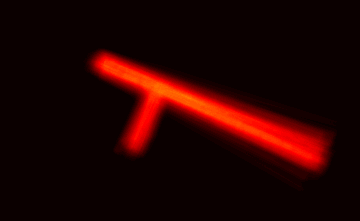
\includegraphics[width=\textwidth, clip, trim=1.2in 0in .2in 0in]{./Localization/IG1_heatmap}
        \caption{Initial Belief}
        \label{heat:first}
    \end{subfigure}
    \hfill
    \begin{subfigure}[b]{0.23\linewidth}
        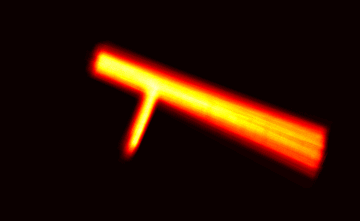
\includegraphics[width=\textwidth, clip, trim=1.2in 0in .2in 0in]{./Localization/IG2_heatmap}
        \caption{1 Measurement}
        \label{heat:second}
    \end{subfigure}
    \hfill
    \begin{subfigure}[b]{0.23\linewidth}
        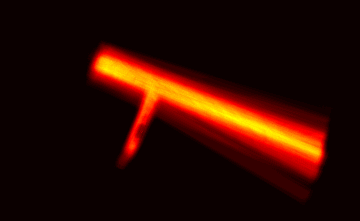
\includegraphics[width=\textwidth, clip, trim=1.2in 0in .2in 0in]{./Localization/IG3_heatmap}
        \caption{2 Measurements}
        \label{heat:third}
    \end{subfigure}
    \hfill
    \begin{subfigure}[b]{0.015\linewidth}
        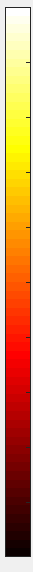
\includegraphics[height=1.3in, width=\linewidth, clip, trim=0.05in 0.2in 0.02in 0.05in]{./Localization/Colorbar}
        \label{heat:colorbar}
    \end{subfigure}
    \hspace*{\fill}
\caption{Heat maps showing information gain}
%% \caption{Heat maps showing information gain of vertical measurements during the localization process.
%% The intensity of every pixel is the normalized expected information gain of a measurement passing through the pixel orthogonal to the image.
%% Initially \subcap{heat:first} probing into the page is likely to miss the part, providing little information.
%% The first measurement reduced the uncertainty such that probing in this direction will more likely contact the part and provide information \subcap{heat:second}.
%% Repeating another measurement in the same place would not provide much information. 
%% \subcap{heat:third}
%% }
\label{fig:Heatmaps}
\end{figure}

Figure \ref{fig:bins} visualizes this binning process. Three measurement actions (arrows) $\maction + \delta_j$ are simulated on three configurations of the part ($\particle[][i] = \text{particle } i$). The intersection between the simulated measurement action and the part determines the measurement value $\measurement_{i,j}$. These measurement values are sorted into bins.


Figure \ref{fig:Heatmaps} visualizes the densely computed information gain for a grid of parallel rays as the ``temperature'' in a heat map. 
Initially \subcap{heat:first} probing into the page is likely to miss the part, so information gain is low for all these measurements and we instead probe sideways. 
After this first measurement \subcap{heat:second} the uncertainty is reduced, and probing into the page is more likely to hit the part and provide information. 
Once this second measurement is performed \subcap{heat:third}, another measurement in the same place will not provide more information.




Adaptations are made to this process to accommodate the two representations as described next:


\subsection{Information for Full-State Representation}
The full-state representation does not maintain a set of particles over just the goal feature, but rather each particle, $\particles$, represents the full $6 \times n$ state.
Using these full-state particles for $\particles[][][G]$ above provides a good metric for localizing every section of the part, but a poor metric for localizing the goal feature.
This metric would often suggest to perform measurements on non-datum features that are irrelevant to the location of the goal feature.
The error in this metric is due to
\begin{align}
  H(\particles[][][G]|\maction) \neq H(\particles|\maction)
\end{align}

One approach is to incorporate domain knowledge when designing the full-state representation, by including only the relevant datums necessary for a particular task. 
Then, any information on this limited full state will be reduction of uncertainty of at least one datum required for the task.
%% Due to the simplicity of this approach, experiments on the Full State Particle Filter presented in section \ref{sec:experiment} use this method of limited the number of sections in the full state.

An approach that does not require pruning irrelevant sections from the full state involves combining particles that produce similar configuration for the goal feature. 
To calculate $H(\particles[][][G]|\maction)$ using particles $\particles$, measurement actions are used to sort the particles into bins as in described in section \ref{subsec:IG}.
Then, particles that produce sufficiently similar goal feature configurations are treated as identical particles when computing entropy, by combining these into groups $\groups$.
\begin{align}
  p(\particles[][L]|\bin_k) &= 
  \frac{\sum_{i,j} \mathds{1}(\measurement_{i,j} \in \bin_k) \mathds{1}(i \in L) \cdot w_i}{W_k}\\
  H(\particles | \bin_k) &= -\sum_L p(\particles[][L]|\bin_k) \log(p(\particles[][L]|\bin_k))  
\end{align}
These group can be constructed by discretizing the space of possible configurations for the goal feature.
An issue which this thesis does not address is the balance of a requiring a reasonably small number of particles while maintaining sufficient density for this descretization of goal feature configuration to produce meaningful group sizes.


\subsection{Information for Independent-State Representation}
The independent-state representation does maintain the set of goal feature particles, $\particles[][][G]$, however additional steps are needed when computing Eq. \ref{Eq:Simulate}.
When simulating $\maction$, the robot will measure some section, $\feature$, of the part.
Simulating the measurement using $\particles[][][\feature]$ is straightforward, but leads to computing $IG(\particles[][][\feature]|\maction)$, which is not the desired metric $IG(\particles[][][G]|\maction)$.


The independent-state representation makes the approximation that the distribution of transformations between sections are fixed and independent, and this approximation is used to achieve the desired metric.  
A temporary set of particles $\tilde \particles^\feature$ is created by sampling transforms $T_G^\feature$ and applying these transforms to $\particles[][][G]$.
$\tilde {\particles[][][\feature]}$ is used in Eq. \ref{Eq:Simulate} to generate sample measurement values $\tilde \measurement_{i,j}$, which are used in the calculation for bin entropy $H(\particles|\bin_k)$.
While the independence approximation could be used again in the calculation of bin probabilities $p(\bin_k)$, this approximation is not needed. 
Measurements $m_{i,j}$ calculated using $\particles[][][\feature]$ are used to calculated $p(\bin_k)$.

%% However, measurements $m_{i,j}$ are also calculated using $\particles[][][\feature]$.
%% These measurements are used to calculate the bin probabilities $p(\bin_k)$.


%%%%%%%%%%%%%%%%%%%%%%%%%%%%%%%%%%%%%%%%%%%%%%%%%%%%%%%%%%%%%%%%%%%%%%%%
\section{Experiments} \label{sec:experiment}

The following experiments validate both the full-state representation approach and independent-state representation approach in simulation. 
The software was implemented in ROS using C++. 
These experiment simulate a specific task which is common in manufacturing: localizing a target location, defined by datums, to drill a hole on an object. 
%PLACEHOLDERS for picture for datum visualization
The datum-based particle filter was simulated on a structural component used in aircraft. This is the same object as used in the original rigid-body particle filter paper\cite{Saund2017}, with adaptations made to allow internal degrees of freedom.
The object is composed of 5 precisely manufactured sections, and tolerance between sections was determined by engineering drawings (for precisely defined features), and educated guesses (for loosely defined relationships). 
%% The tolerance is modeled by a distribution over $SE(3)$ transforms, as described in Section \ref{sec:datum}. 

\subsection{Measurement Selection}

The target hole is localized by measuring its referenced datums. 
Specifically, the pose of the hole feature (green cylinder) in figure \ref{fig:FullBelief} is defined by an offset distance from the top and right sections shown in figure \ref{fig:Overview:CAD}, and the axis of the hole is orthogonal to the front plane. 
%% Since the task is to localize the position to drill the hole, measurements are allowed only on the given 5 sections. 
The hole does not exist yet, and thus cannot be measured directly.
In order to localize the hole location precisely without direct measurement on the hole, it is assumed that the transformations between the target location and its defining datum sections have very small uncertainty along some dimensions, e.g. the vertical distance between the center of the hole and the top plane.

At each step, the measurement is simulated using ray-mesh intersection algorithms\cite{Saund2017}. 
%% Each measurement is assumed to have a small measurement error (0.2mm). 
Potential measurement actions are sampled in the workspace. 
The information gain for each measurement is calculated based on the current estimated pose of each section.
For each measurement performed, candidate actions are evaluated until 500 actions with non-zero information gain have been modeled.
Only the measurement action with the largest expected information gain is ``performed'' in simulation and used to update the belief. 
\begin{figure}
  \centering
  \begin{tikzpicture}
    %% \node (img) {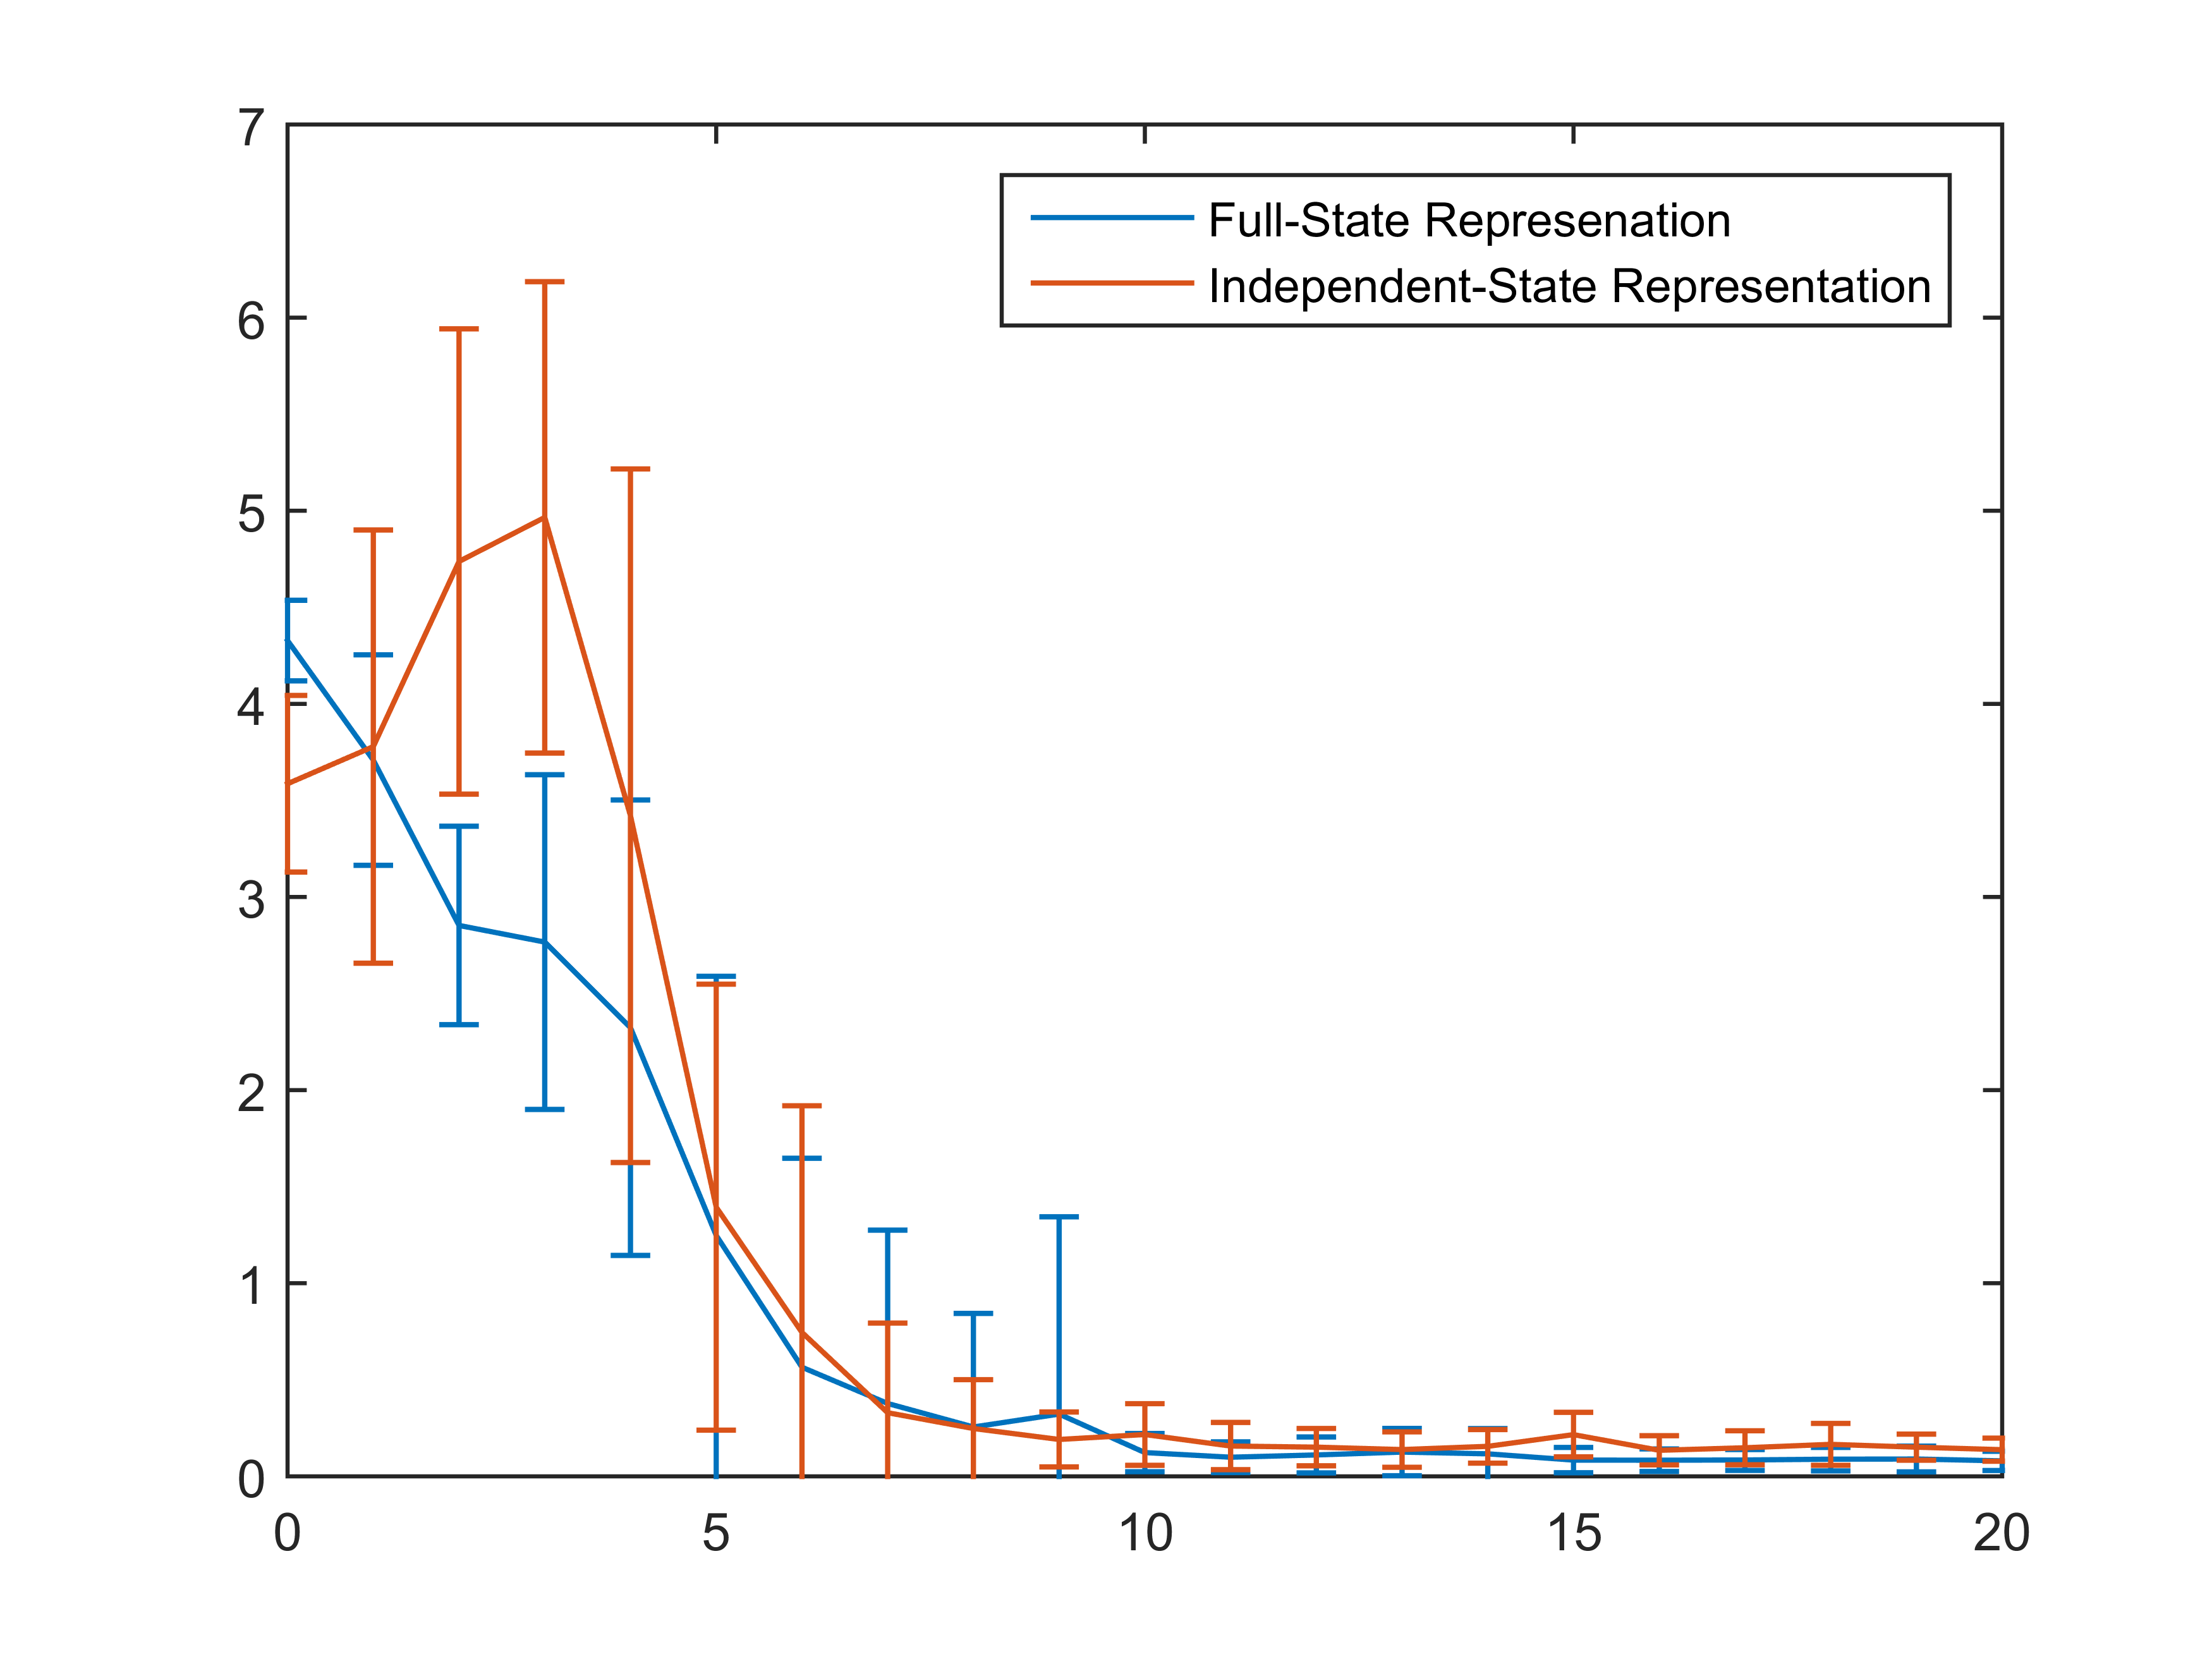
\includegraphics[width=.3\linewidth, clip, trim=1.5in 3.3in 1.5in 3.3in]{./Localization/translational_error}};
    \node (img) {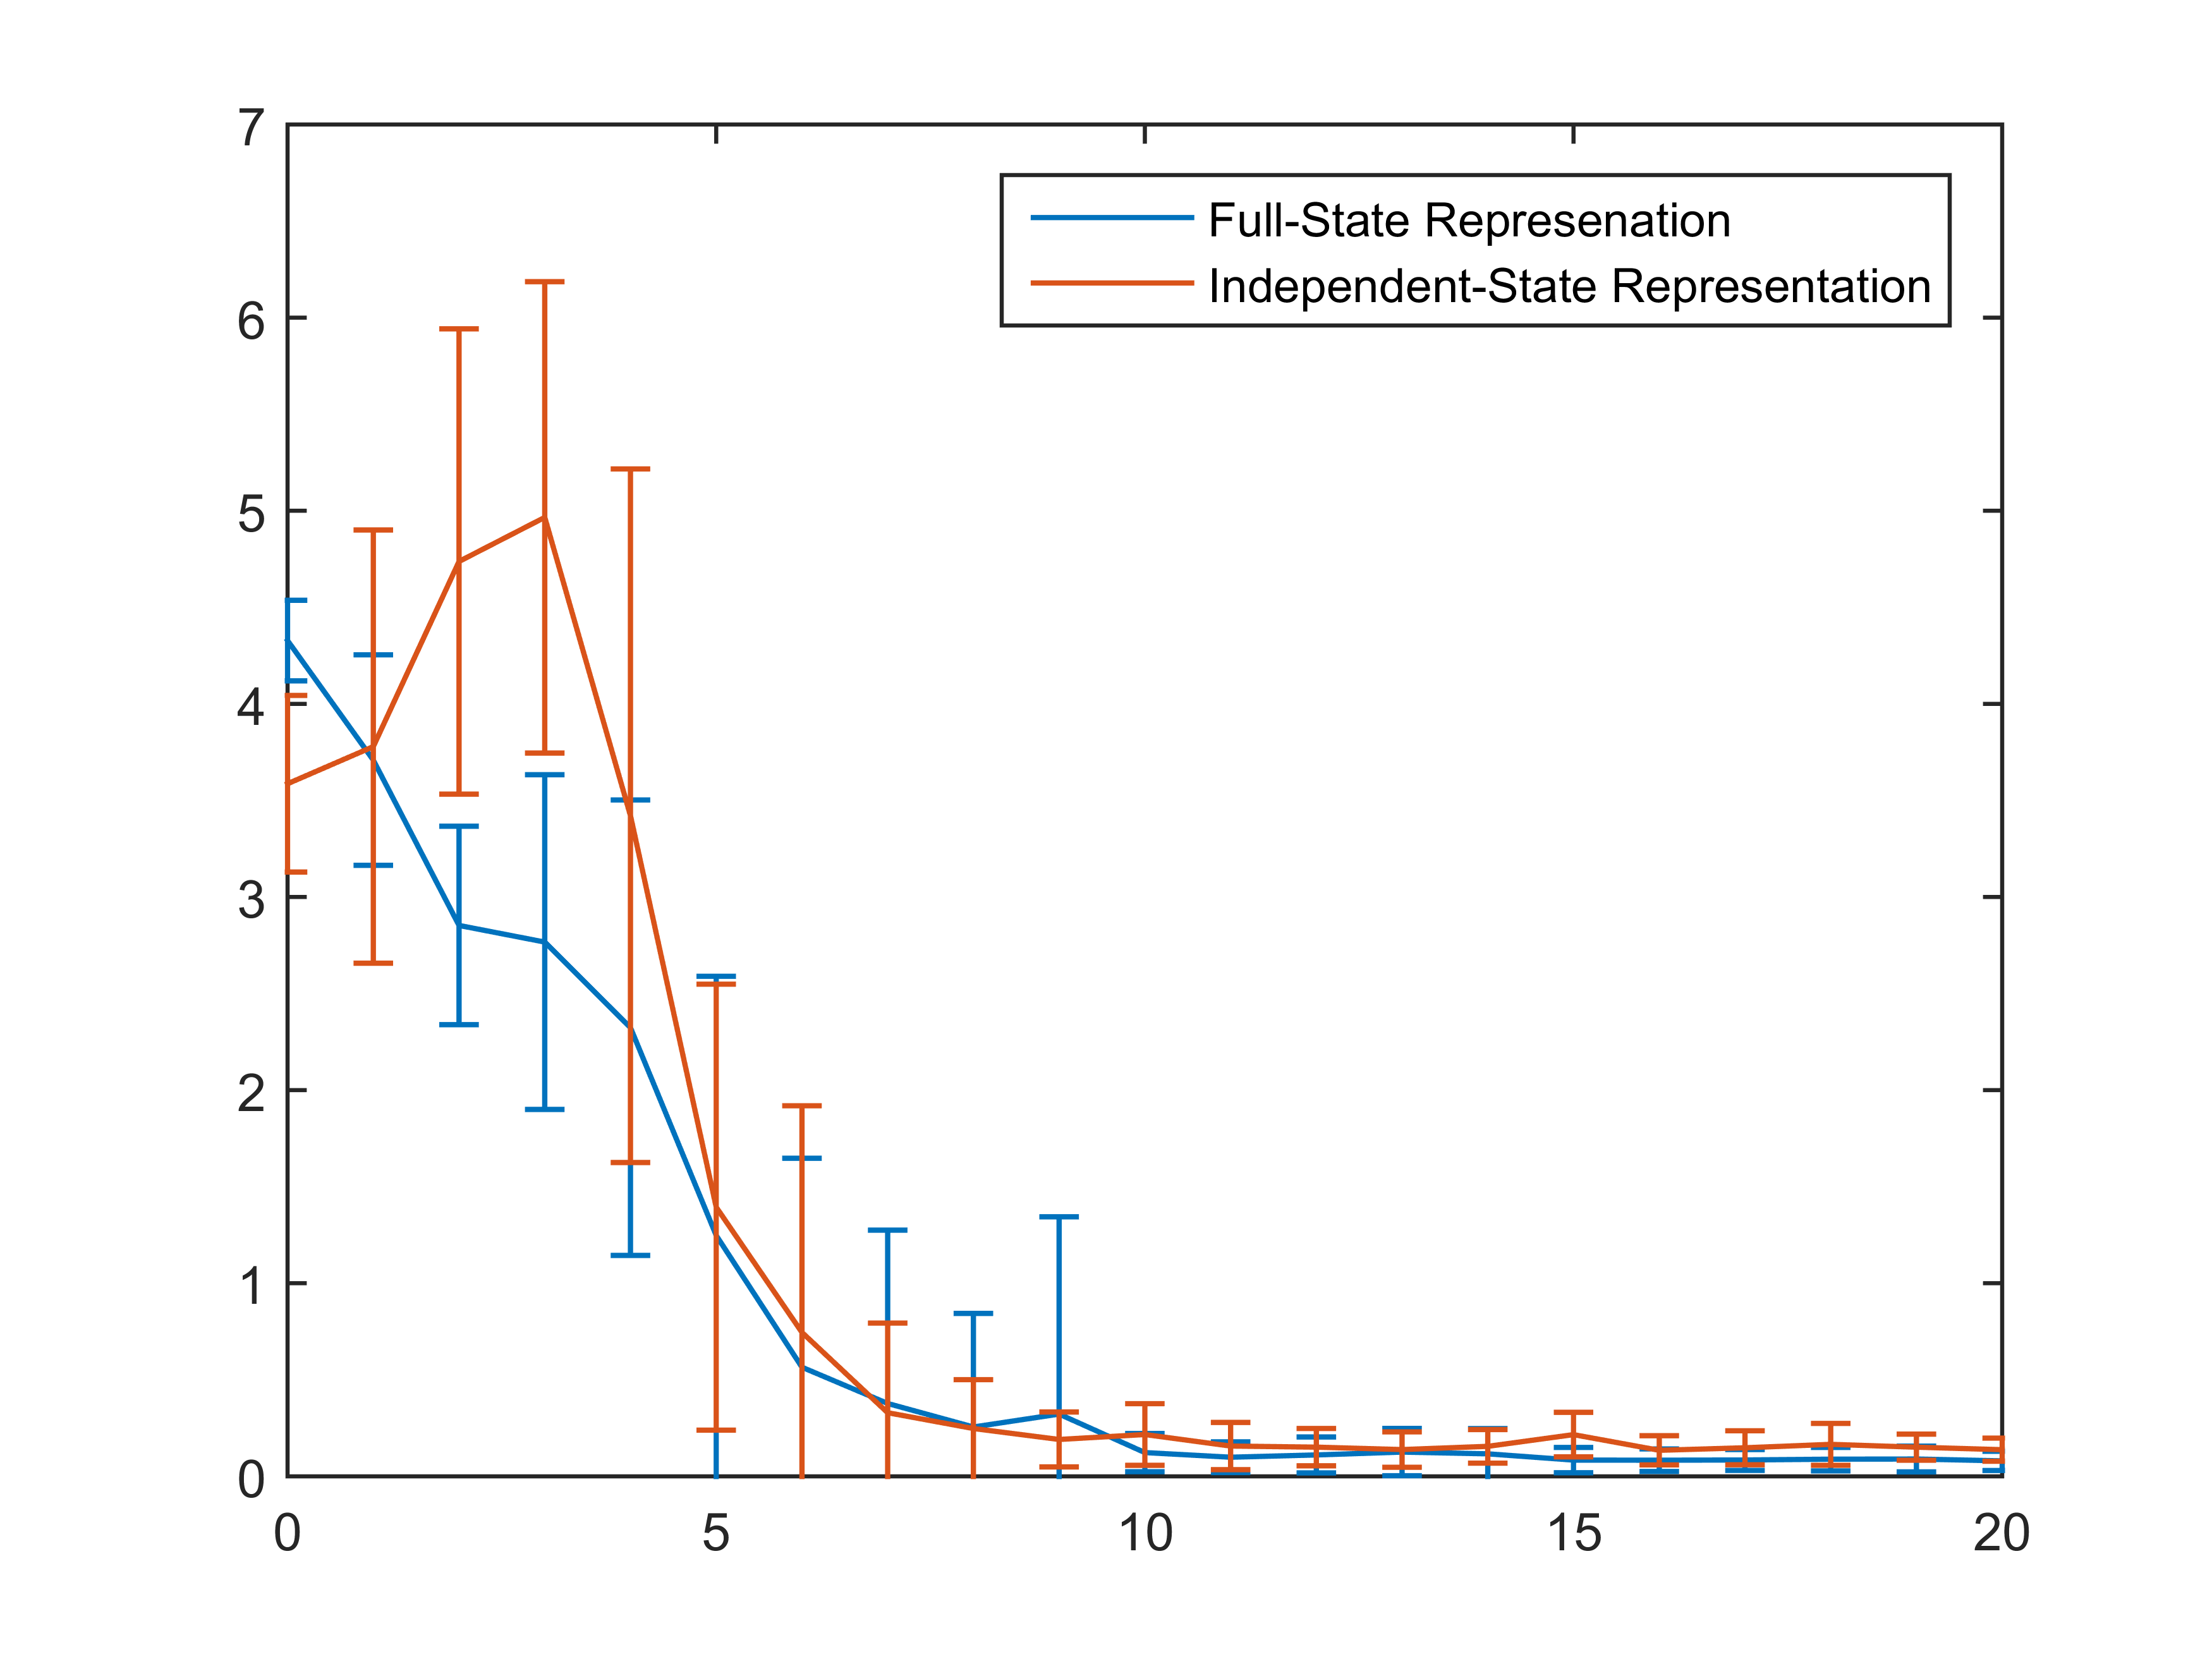
\includegraphics[width=.7\linewidth]{./Localization/translational_error}};
    \node[left=of img, node distance=0cm, rotate=90, anchor=center,yshift=-1cm] 
         {Translational Error (cm)};
  \end{tikzpicture}
  \begin{tikzpicture}
    \node (img) {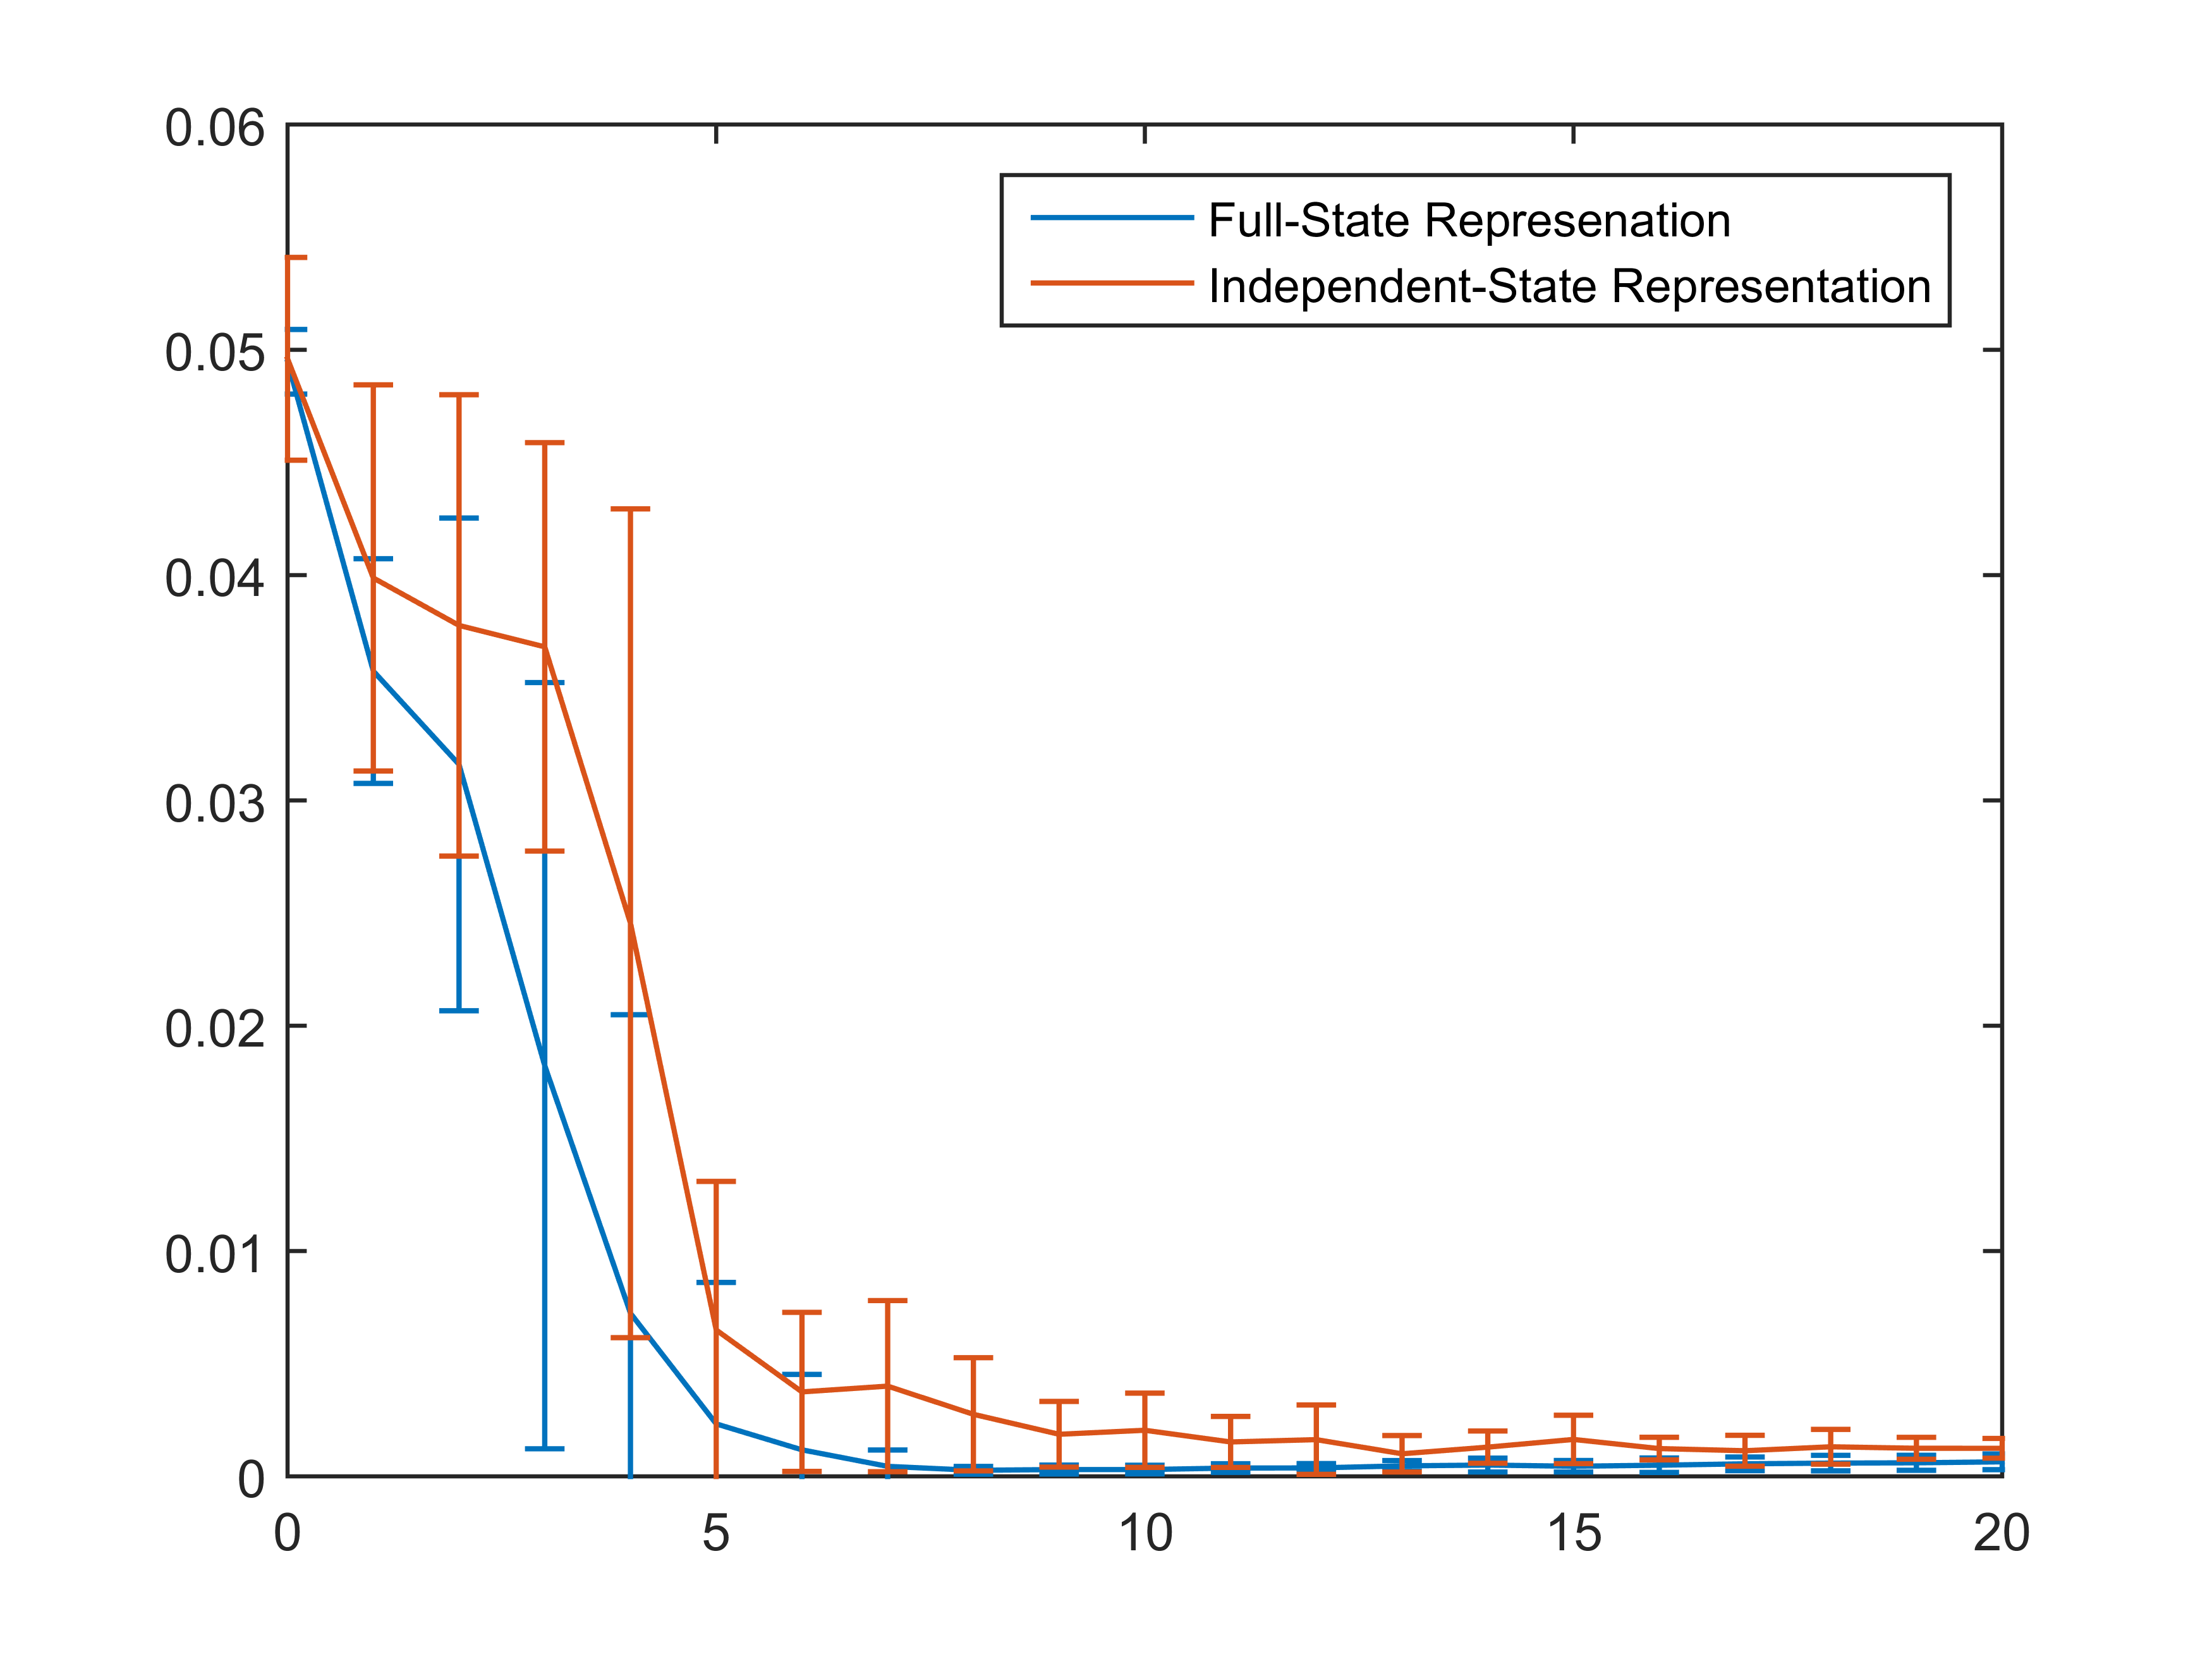
\includegraphics[width=.7\linewidth]{./Localization/rotational_error}};
    \node[left=of img, node distance=0cm, rotate=90, anchor=center,yshift=-1cm] 
         {Rotational Error (rad)};
         \node[below=of img, node distance=0cm, yshift=1.2cm] 
              {Measurement Number};
  \end{tikzpicture}
  %% \begin{tikzpicture}
  %%   \node (img) {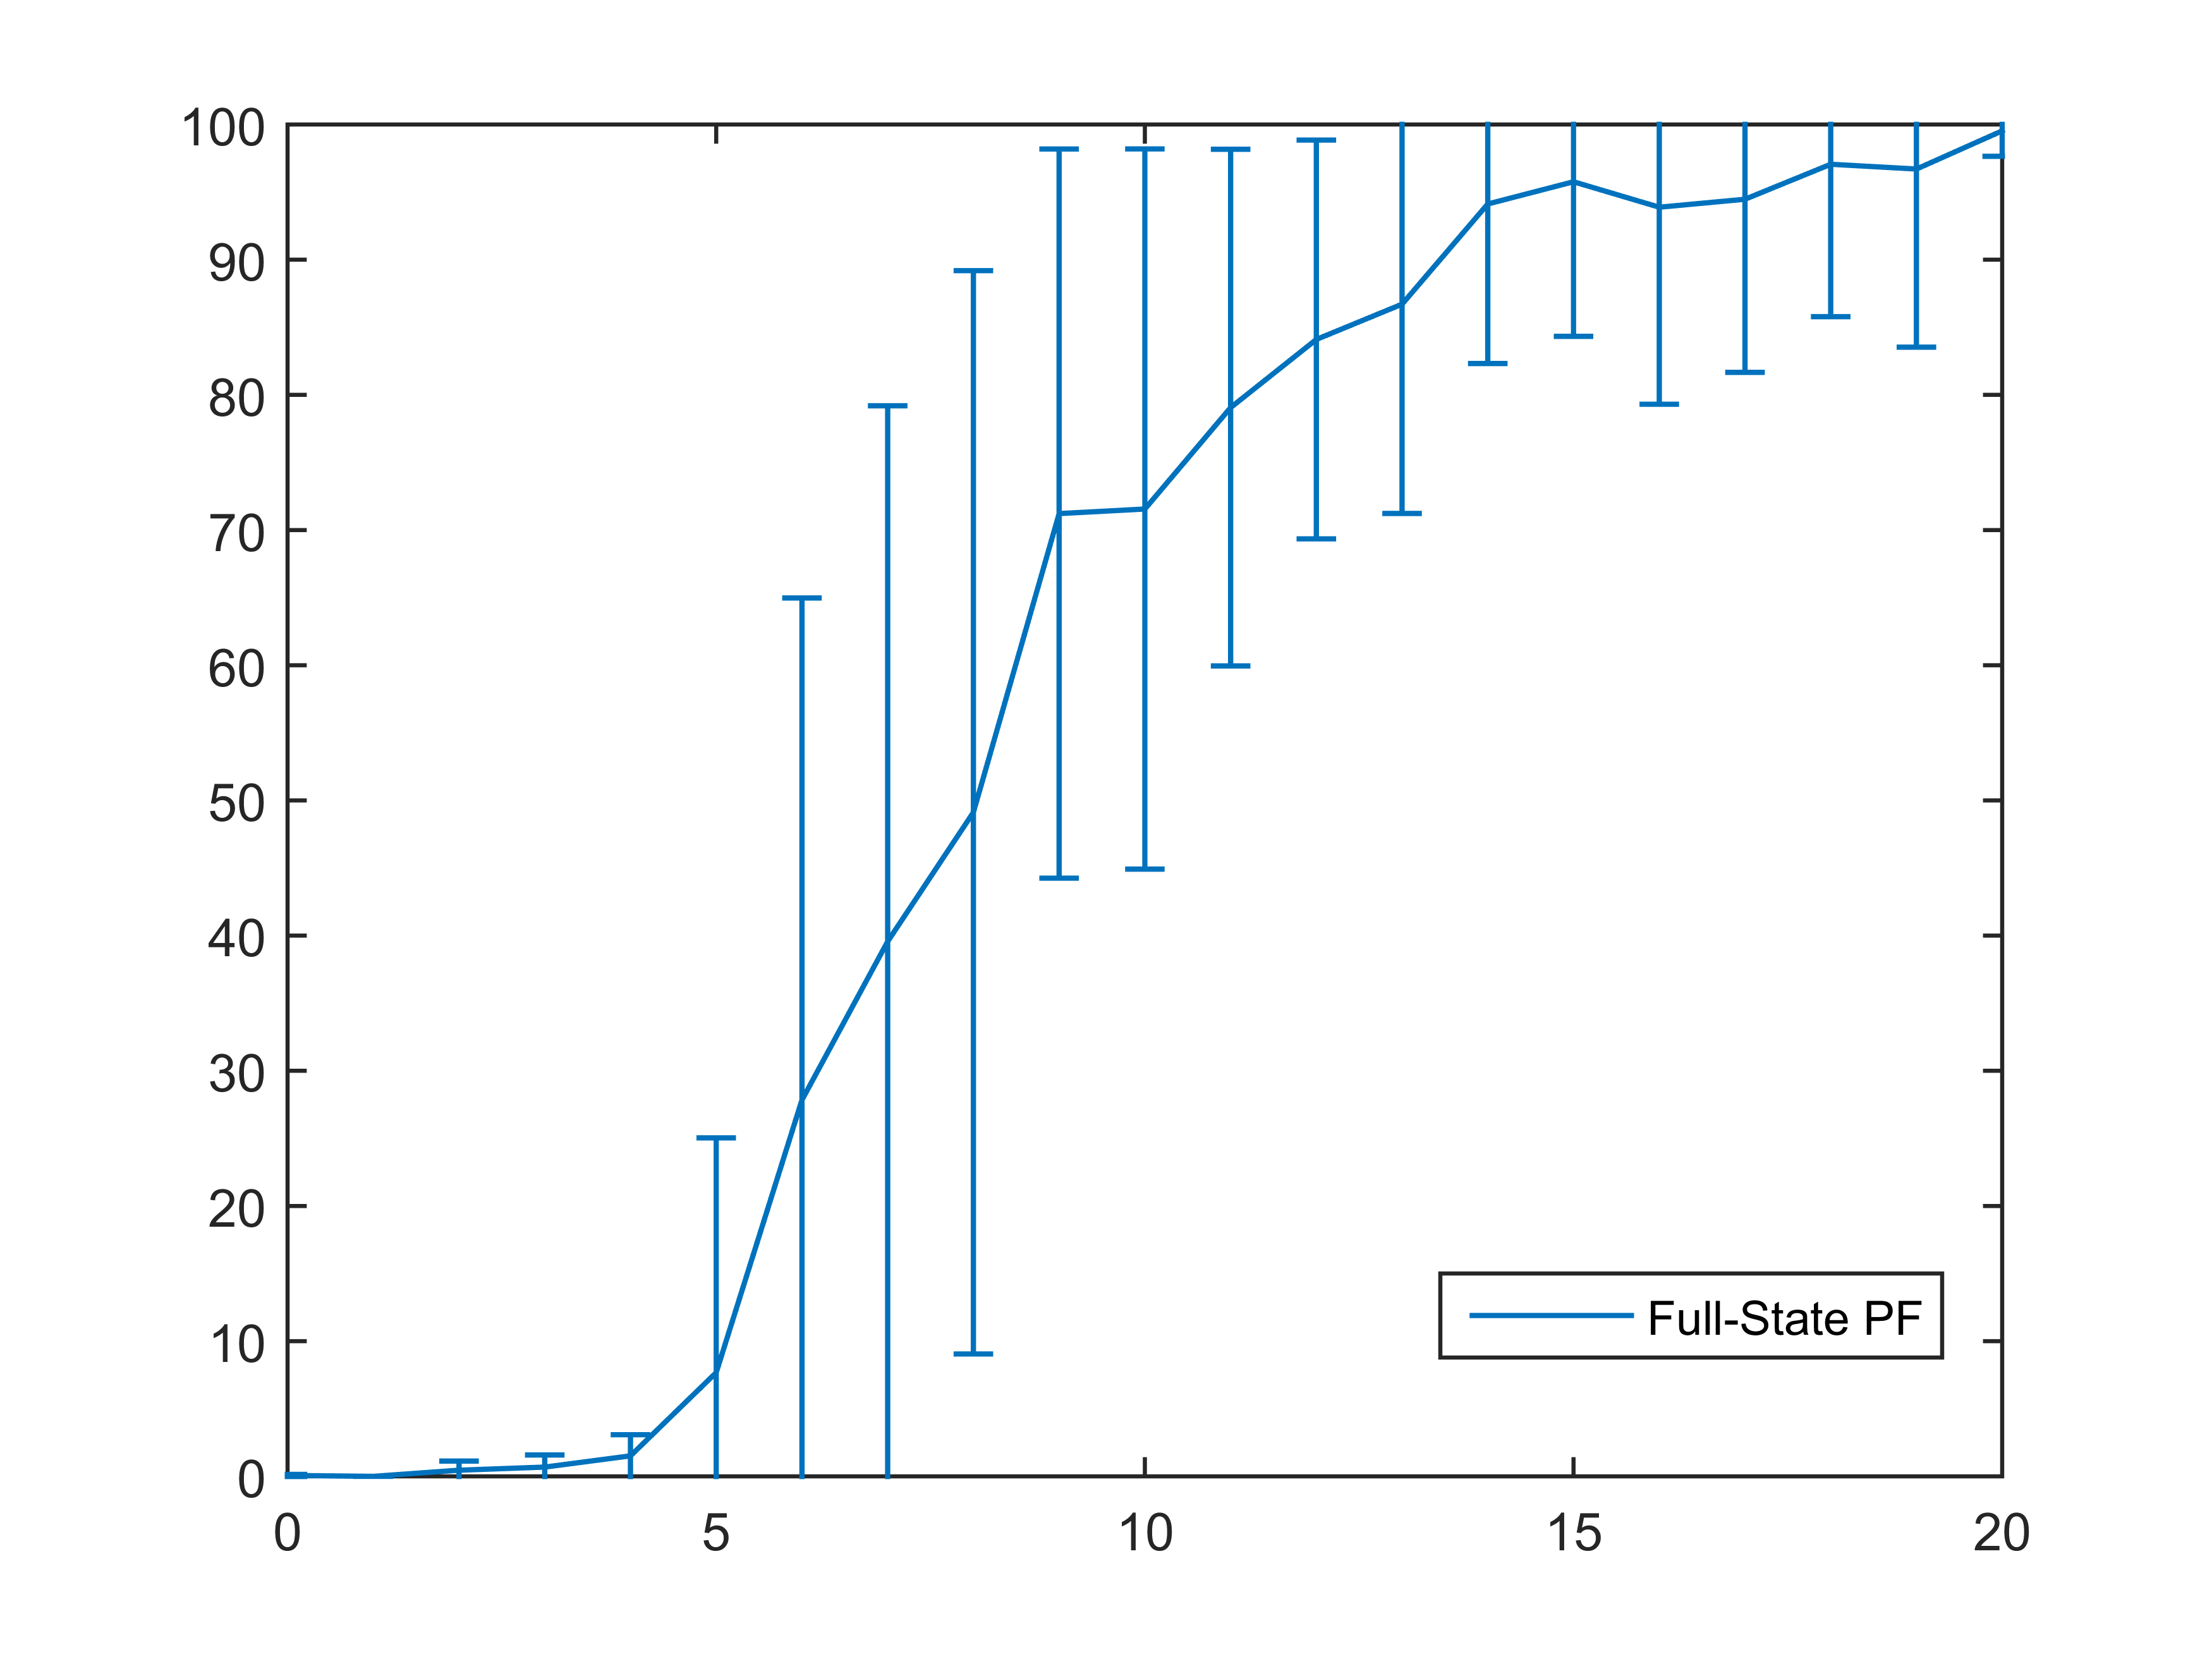
\includegraphics[width=3in, clip, trim=0in 0in 0in 0in]{./Localization/fitted_rate}};
  %%   \node[left=of img, node distance=0cm, rotate=90, anchor=center,yshift=-1cm] 
  %%       {Fitted Rate (\%)};
  %%   \node[below=of img, node distance=0cm, yshift=1.2cm] 
  %%       {Measurement Number};

  %% \end{tikzpicture}

  \caption{Comparison of the accuracy of the update step when using full-state particle filter and independent-state particle filter}
  \label{fig:Simulation}
\end{figure}

\subsection{Simulation Results}

Both proposed approaches are compared in similar settings.
A total of 20 measurements are simulated during each trial. 
For the full-state representation, a maximum of 800 particles are used. For the independent-state representation, a maximum of 500 particles are used for each section.
The simulation uses 5 mesh models for different sections. 
%% For the simulation, the radius of the target hole is fixed to $1cm$ and the depth is $3.5cm$. 
After each update, the average estimated pose of the hole is computed by averaging the hole poses produced from all particles. 

Figure \ref{fig:Simulation} shows the comparison between the full-state particle filter and independent-state particle filter. 
Translational error and rotational error are defined between the estimated pose of the hole and its true state. 
%% In addition, we define a metric for this specific task: the percentage of the hole particles that lead to a pose with no intersection between the walls of the estimated hole and a cylinder with a radius equals to $80\%$ of the hole radius fitted along the center line of the hole at the true state. 
%% When the \textit{fitted rate} equals $100\%$, all particles will result in the case that fitted cylinder will completely pass through the hole at each estimated pose without any intersection.
From the simulation, the errors of the estimated pose decreases rapidly for both approaches after each new measurement is applied on the system. 
%% The fitted rate also increases.



\end{document}
